\clearpage
\section[Comment explorer les sorties de SimFeodal ?]{Comment explorer les sorties de SimFeodal ?%
\sectionmark{Explorer les sorties}}\label{sec:explorer-sorties-simfeodal}

	Pour évaluer, de manière approfondie, une expérience (voir \cref{tbl:hierarchie-simulations}) d'un modèle tel que SimFeodal, il est nécessaire de passer en revue de nombreux indicateurs de sortie de simulation.
	Cette évaluation ne vise pas à produire une \og note\fg{} unique et synthétique, mais plutôt à tester la capacité de l'expérience à reproduire les dynamiques que le modèle chercher à reproduire.
	Il ne s'agit pas, à proprement parler, d'une validation du modèle, au sens quantitatif où on pourrait l'entendre.
	On vise plutôt à explorer le comportement du modèle en fonction des mécanismes et valeurs de paramètres choisis.
	Cela aboutit donc sur un jugement qualitatif sur la capacité du modèle à reproduire les dynamiques souhaitées.
	Pour mener cette exploration, il convient d'utiliser des outils adaptés, c'est-à-dire de disposer de solutions techniques permettant le calcul et l'affichage des indicateurs à partir des données produites par le modèle.
	
	Dans le travail mené autour de SimFeodal, plusieurs solutions ont été utilisées au cours des différentes étapes de construction du modèle.
	La restitution purement chronologique de ces solutions ne revêt pas d'intérêt propre, mais les contraintes accumulées au cours de la construction du modèle ainsi que les choix devant permettre de les dépasser nous paraissent très largement génériques et généralisables.
	
	La succession de choix d'outils d'explorations se justifie par les verrous dans l'exploration que chacun de ces outils a permis de débloquer.
	Cela dresse par là-même un portrait des solutions méthodologiques d'exploration de données de simulations dont on peut faire usage selon les contraintes générales des modèles.

	\subsection{Observation en direct ou \textit{a posteriori}}\label{subsec:observation-a-posteriori}

	Classiquement, le premier réflexe d'un modélisateur, du moins pour les modèles à base d'agents, est de définir des sorties graphiques pour accompagner son modèle.
	Les différentes plate-formes de modélisation agent mettent d'ailleurs régulièrement en avant les possibilités de représentations qu'offrent leurs environnements\footnote{
		Voir par exemple les collections de visualisations sur les pages d'accueil de Gama (\href{https://gama-platform.github.io/}{https://gama-platform.github.io/}), de NetLogo (\href{https://ccl.northwestern.edu/netlogo/}{https://ccl.northwestern.edu/netlogo/}), de GeoMASON (\href{https://cs.gmu.edu/~eclab/projects/mason/extensions/geomason/}{https://cs.gmu.edu/$\sim$eclab/projects/mason/extensions/geomason/}) ou encore de Repast (\href{https://repast.github.io/screenshots.html}{https://repast.github.io/screenshots.html}).
	}.
	Visualiser le déroulement d'un modèle \og en direct\fg{} (\og \textit{online}\fg{} dans \cite{grignard_agent-based_2017}), c'est-à-dire au sein de la plate-forme de simulation et au cours l'exécution du modèle, offre ainsi de nombreux avantages : évaluation visuelle du niveau de ségrégation (et de son évolution) dans une implémentation du modèle de Schelling ; visualisation de cohérence du déplacement des nuées d'oiseaux dans un modèle de type \og Flocks\fg{} \autocite{reynolds_flocks_1987} ; ou encore suivi d'un indicateur dans le temps -- la quantité de ressources collectées -- dans un modèle de type \og Sugarscape\fg{} \autocite{epstein_growing_1996}.
	
	Il est à noter que dans le cadre du développement d'un modèle de simulation, l'implémentation du modèle et de son interface graphique sont étroitement liées.
	D'une part, la plateforme de modélisation choisie contraint fortement le type et la diversité des représentations.
	Gama et GeoMASON, par exemple, proposent des modes de visualisation de données géographiques bien plus avancés que NetLogo ou Repast.
	L'interface graphique développée pour chaque modèle est donc largement influencée par la plateforme de simulation dans laquelle il est exprimé.
	D'autre part, dans la plupart de ces plateformes de simulation, l'interface graphique est implémentée au même niveau que le code-source du modèle en lui-même.
	Dans Netlogo et Gama par exemple, l'interface graphique est programmée directement dans le modèle en lui-même, en se basant sur les variables qui y sont déclarées.
	Il n'est donc pas possible de créer une interface graphique générique au sein des plateformes de simulation, laquelle pourrait s'appliquer à plusieurs modèles différents.
	Il est nécessaire, pour chaque modèle, de reconstruire l'interface depuis les briques de bases proposées par les plateformes, c'est-à-dire un ensemble de primitives graphiques permettant de composer une interface intégrée au modèle.

	Dans l'exploration de SimFeodal, la création en direct de quelques graphiques correspondant à des indicateurs étudiés permet d'assurer un rôle de filtrage, grossier, à l'exécution d'une expérience, c'est-à-dire de l'ensemble des réplications nécessaires à son évaluation.
	Après une modification du code-source du modèle, et avant de lancer de nombreuses simulations, on exécute quelques simulations \og manuellement\fg{}.
	On s'assure alors, en direct, que les indicateurs affichés ne présentent pas de caractères aberrants.
	Cela permet de vérifier, avant de lancer des calculs plus conséquents, que le déroulement de la simulation semble cohérent, c'est-à-dire, le plus souvent pour des modifications mineurs du modèle,  qu'un \textit{bug} n'a pas été introduit involontairement.
	
	Le recours à ce type de visualisation en direct des simulations ne peut toutefois être généralisé, c'est-à-dire sorti de son rôle de pré-filtre, en raison de deux principales contraintes.

	La première contrainte, déjà évoquée plus haut, est que le modèle SimFeodal est fortement stochastique.
	Dès lors, la visualisation des indicateurs d'une simulation particulière n'est pas suffisante pour estimer le comportement du modèle.
	En conséquence, les indicateurs choisis pour l'évaluation de SimFeodal prennent presque tous en compte la variabilité des résultats induite par l'exécution de réplications.
	Certains environnements techniques\footnote{
	Gama dans sa dernière version (1.8) par exemple, voir\\ \href{https://gama-platform.github.io/wiki/RunSeveralSimulations.html}{https://gama-platform.github.io/wiki/RunSeveralSimulations.html}.
	} permettent toutefois de mener concomitamment plusieurs réplications d'un même modèle et de visualiser directement pendant l'exécution les résultats agrégés des réplications.
	Cette première contrainte, liée au besoin d'analyser des réplications plutôt que des exécutions isolées, peut donc être dépassée en adaptant l'implémentation du modèle pour faire usage de ces capacités de multi-simulation.

	La seconde contrainte est cruciale dans le cas de SimFeodal et invalide l'usage des méthodes de visualisation en direct.
	On l'a vu, l'exploration des sorties de simulation du modèle repose sur la consultation systématique de plusieurs indicateurs, dont le nombre peut se révéler important pour une analyse approfondie.
	
	Tout d'abord, il est concrètement difficile de représenter tous ces indicateurs au sein de l'interface graphique d'une plate-forme de simulation agent, comme on peut le remarquer, par exemple en \cref{fig:simfeodal_gui_indicateurs} : l'espace occupé par les quelques indicateurs temporels et numériques affichés est déjà important et rend l'interface d'ensemble complexe.
	De plus, et c'est sans doute le verrou majeur, la temporalité de l'exécution d'une simulation -- ou même des réplications nécessaires -- est bien plus courte que celle requise pour la compréhension des résultats produits.
	Une simulation requiert ainsi au maximum quelques minutes.
	Pour pouvoir examiner tous les indicateurs pendant cette durée, il serait nécessaire de mettre la simulation en pause régulièrement, presque à chaque pas de temps.
	On disposerait alors d'un temps suffisant pour observer les indicateurs (organisés en onglets dans l'interface visible dans la \cref{fig:simfeodal_gui_indicateurs}).
	L'analyse des indicateurs de sortie de simulation demandent en effet un examen approfondi, et non simplement superficiel, pour pouvoir juger de l'adéquation de ce que ces indicateurs représentent vis-à-vis des attentes thématiques.
	
	Cette contrainte est renforcée par la pratique d'évaluation que la plupart des chercheurs mobilise.
	L'évaluation n'est pas une étape unique et finie, il est utile de pouvoir revenir sur les résultats à différents moments.
	Cela est par exemple nécessaire quand il s'agit de comparer de nouveaux résultats produits à ceux générés par des expérimentations antérieures.
	On ne peut alors se contenter d'évaluations en direct, même en y consacrant un temps important, simplement parce que par nature, ces évaluations seront à reproduire en plusieurs occasions, et qu'il ne serait alors pas rationnel de relancer, à chaque fois, de nouvelles simulations correspondant à des configurations de paramètres et de mécanismes déjà éprouvées.
	
	Un dernier élément contribue à la difficulté de se baser sur une évaluation en direct : en plus du chercheur, amené à revenir de multiples fois sur les résultats d'une expérience, un modèle co-construit peut être évalué par plusieurs chercheurs différents.
	C'est d'autant plus fréquent en situation d'interdisciplinarité, où les points de vue de chacun des membres sont complémentaires et nécessaires.
	Sauf à faire preuve d'une discipline exacerbée, par exemple en réalisant l'ensemble du travail d'évaluation uniquement en séances de travail simultanées et collectives, l'évaluation par plusieurs personne demande que chacun puisse mener ces analyses selon ses propres temporalités.
	En choisissant de baser l'évaluation d'un modèle uniquement sur une analyse en direct, il faudrait alors que chaque chercheur, à chaque fois qu'il souhaite évaluer une même expérience, ré-exécute le modèle de nombreuses fois.
	Cela serait naturellement possible, mais constituerait clairement un gâchis certain de ressources.
	
	L'évaluation d'un modèle interdisciplinaire et exploratoire ne peut donc que difficilement être réalisé en direct, qui plus est quand elle demande de faire appel, dans un cadre de co-construction, à plusieurs points de vue hétérogènes.
	Les modalités mêmes de l'exploration des sorties d'un modèle à évaluation visuelle requièrent donc que les indicateurs soient visibles et explorables à des temporalités différentes, par des chercheurs différents, depuis des lieux divers.
	
	Il est donc indispensable que les indicateurs soient enregistrés et consultables simplement à tout moment, ce qui élimine de fait la visualisation des indicateurs en direct pendant l'exécution des simulations comme unique méthode d'exploration du comportement des modèles exploratoires et descriptifs.
	
	
	\begin{figure}[H]
		\captionsetup{width=\linewidth}
		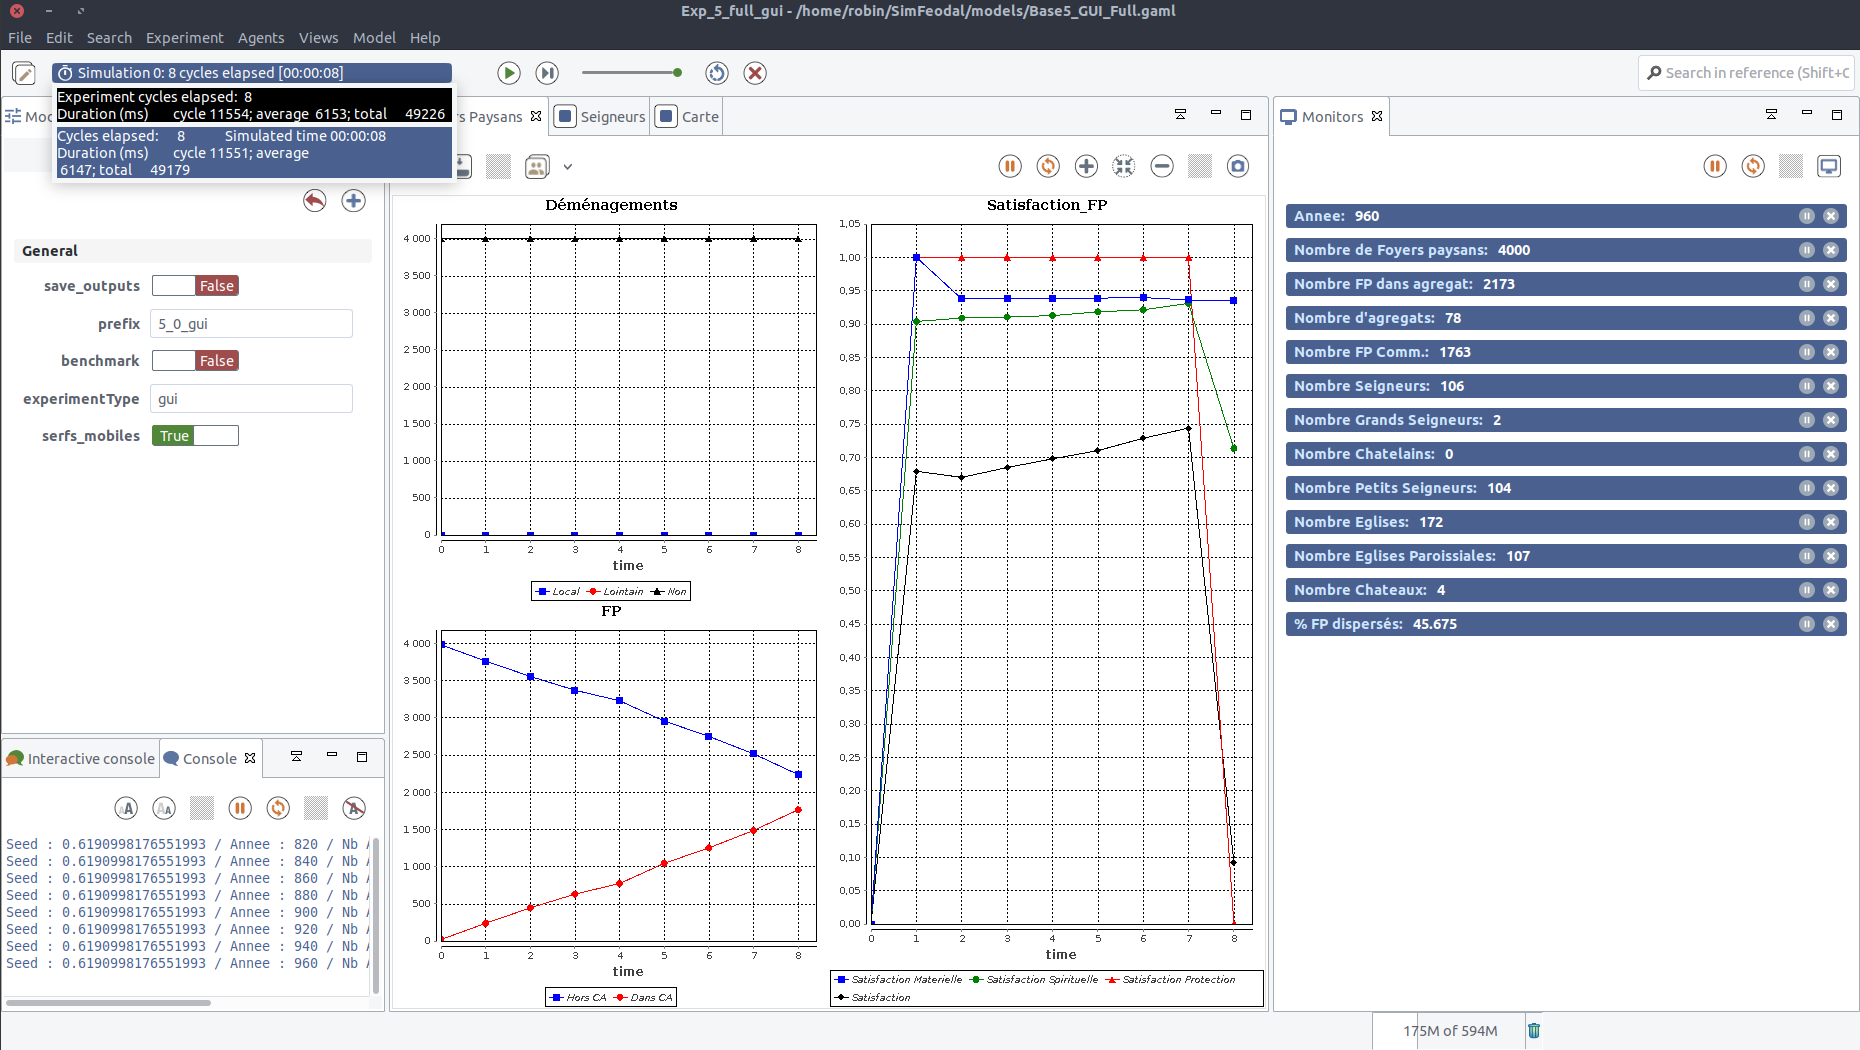
\includegraphics[width=\linewidth]{img/SimFeodal_GUI_FP.png}
		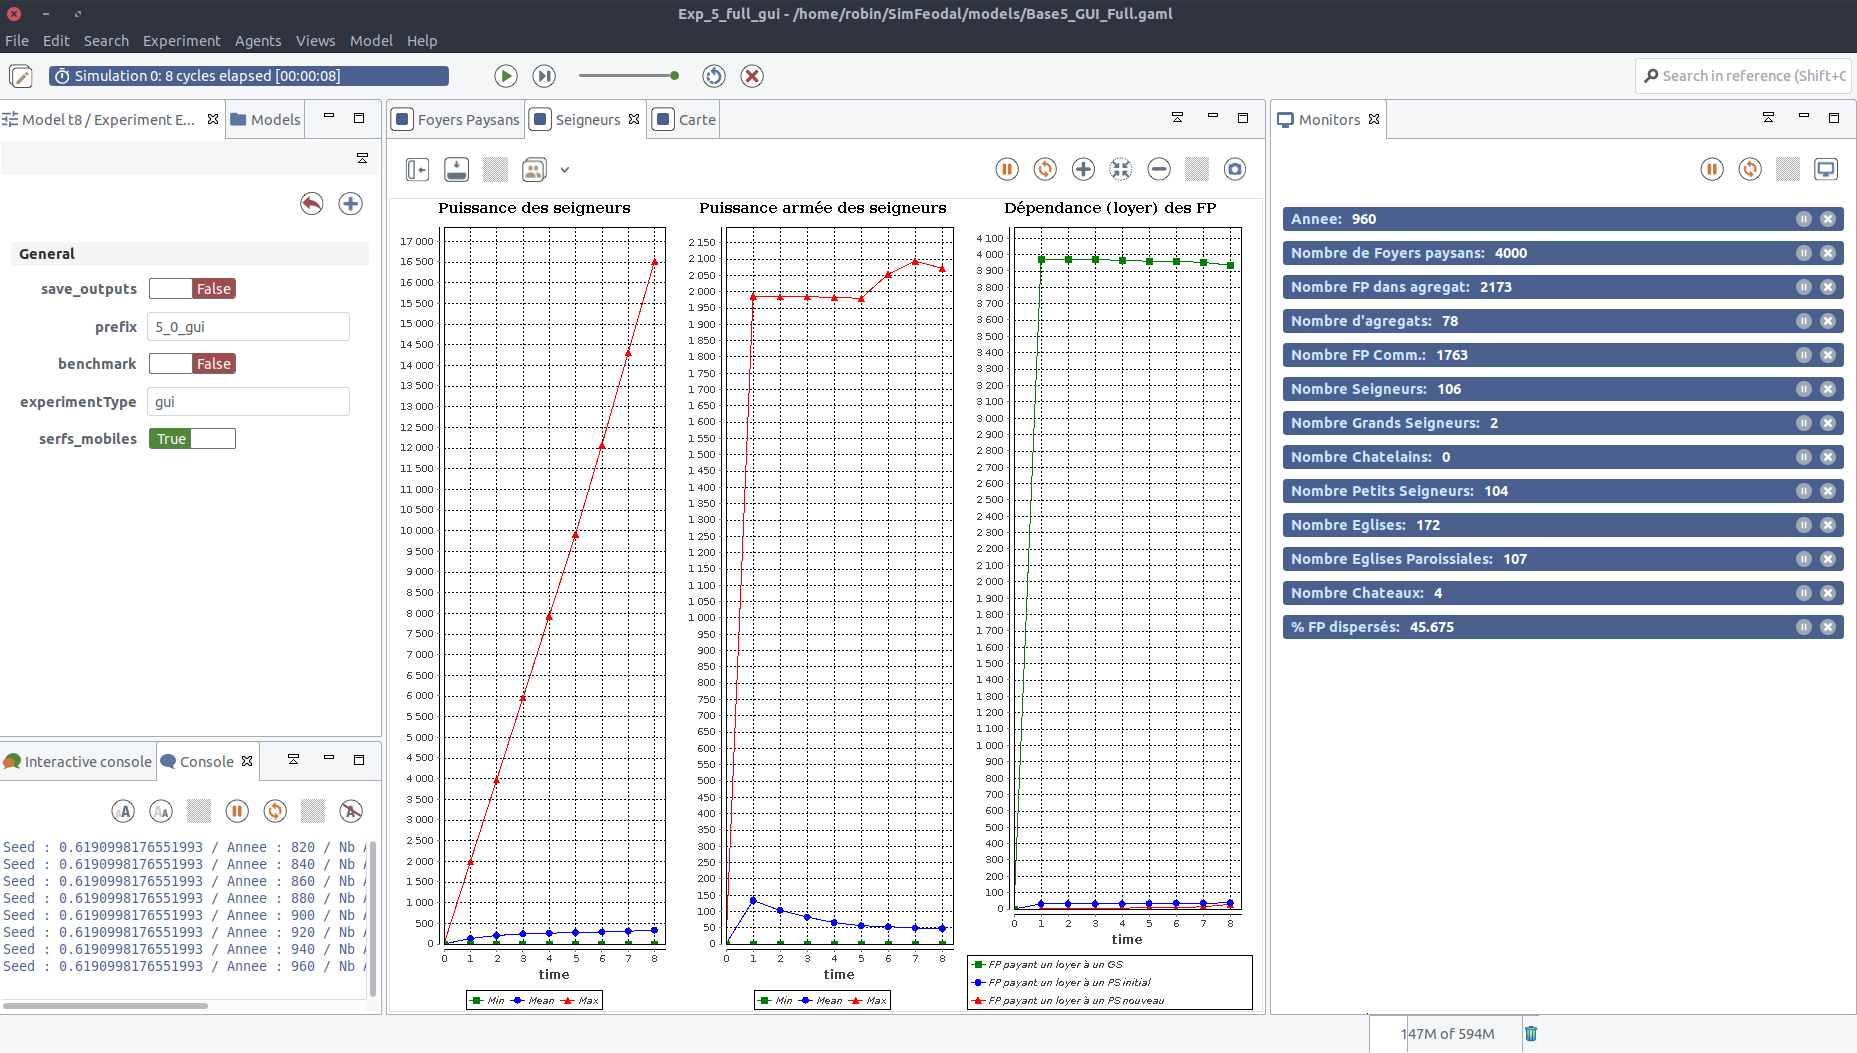
\includegraphics[width=\linewidth]{img/SimFeodal_GUI_seigneurs.png}
		\caption{Indicateurs intégrés à l'interface graphique interne de SimFeodal.
		Dans ces captures d'écrans, il s'agit d'indicateurs liés aux foyers paysans et aux seigneurs.}
		\label{fig:simfeodal_gui_indicateurs}
	\end{figure}
	
	La visualisation en direct n'est donc pas mobilisable en tant que méthode d'évaluation principale, mais elle peut tout de même, comme dans un usage très classique, être utilisée comme un outil de validation interne pour tester chaque modification dans les valeurs de paramètres, remplissant alors le rôle de \og préfiltre\fg{} décrit auparavant.
	Visualiser une seule simulation, avant d'en exécuter les réplications nécessaires, permet ainsi déjà de vérifier que les modifications apportées dans les valeurs de paramètre ou dans les mécanismes n'ont pas entraîné l'apparition de \textit{bugs} ou d'incohérences immédiatement visibles.

	Nous avons donc choisi de développer une interface graphique, très sommaire mais permettant des allers-retours rapides entre l'implémentation et l'exécution, au sein de l'implémentation de SimFeodal.
	Cette interface n'affiche qu'un nombre réduit d'indicateurs (\autoref{fig:simfeodal_gui_indicateurs}), ainsi qu'une représentation cartographique (\autoref{fig:simfeodal_gui_carte}) utile à une analyse rapide du comportement d'ensemble du modèle.

\begin{figure}[H]
	\captionsetup{width=\linewidth}
	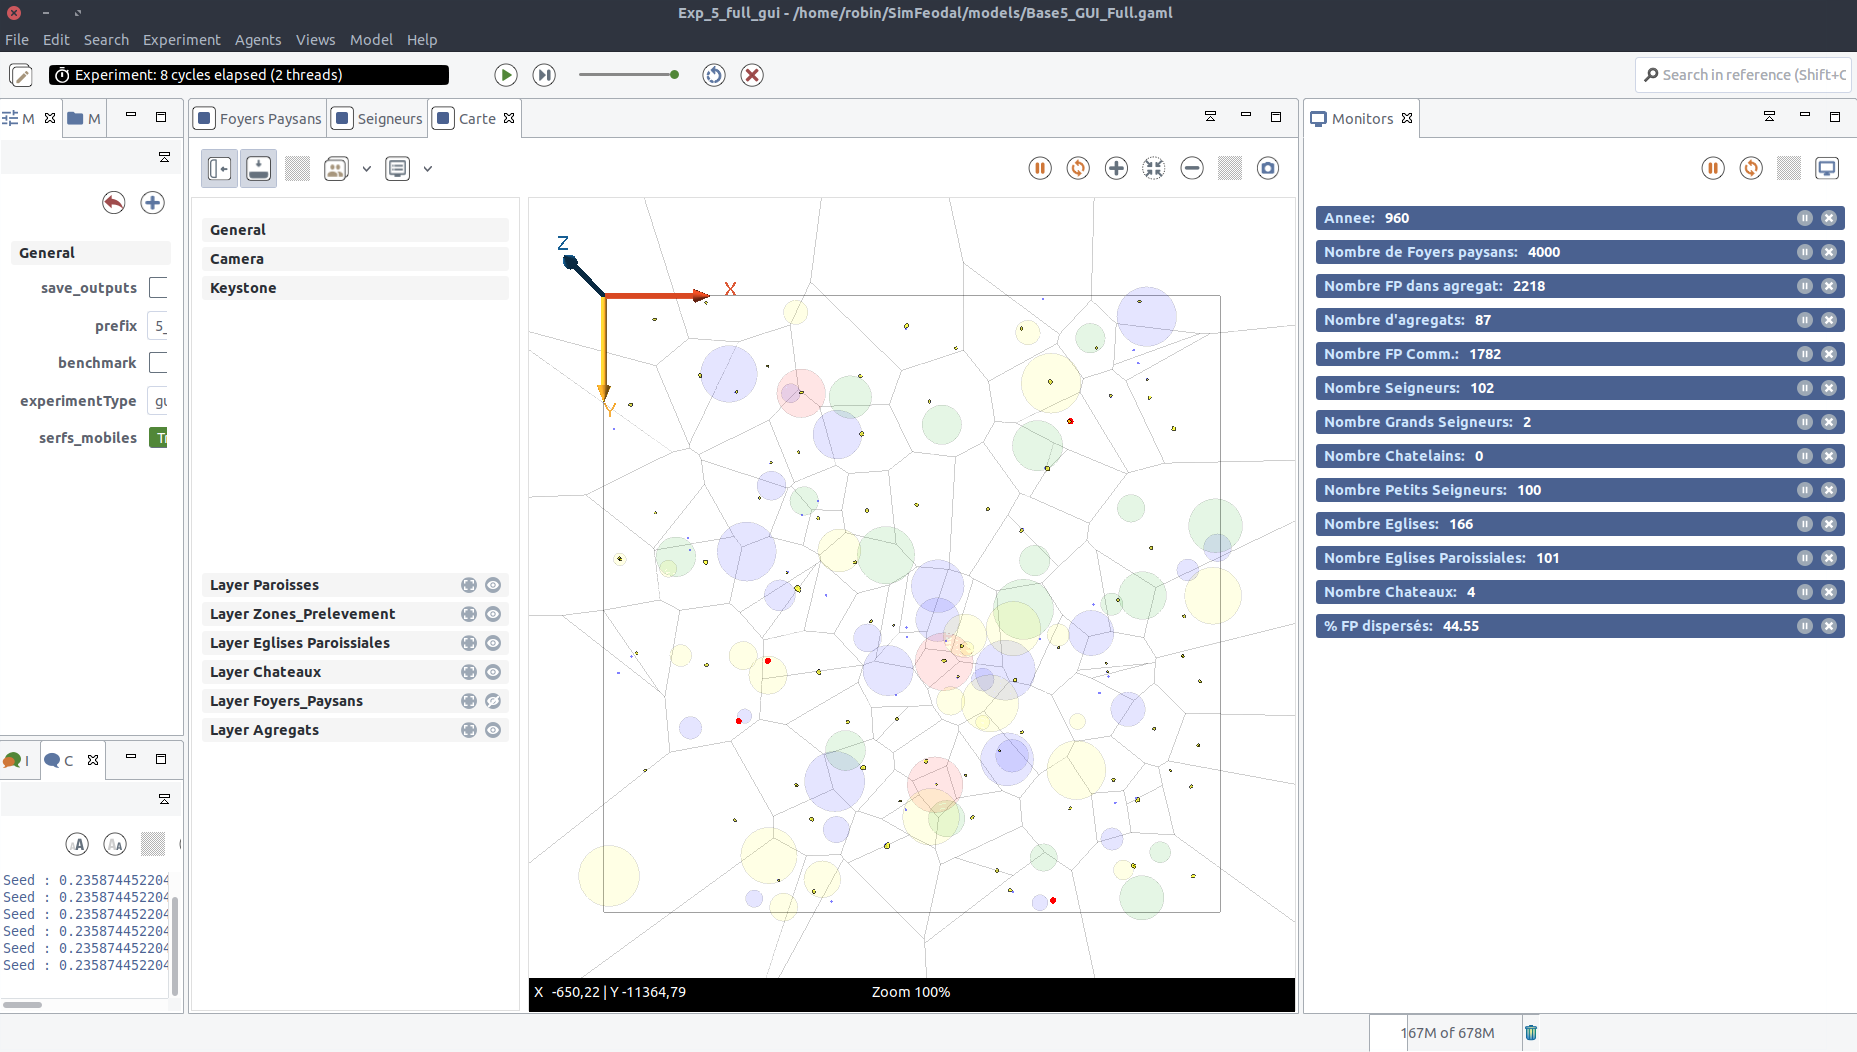
\includegraphics[width=\linewidth]{img/SimFeodal_GUI_carte.png}
	\caption{Visualisation intégrée à l'interface graphique interne de SimFeodal : cartographie synthétique de l'espace modélisé.}
	\label{fig:simfeodal_gui_carte}
\end{figure}

	Ces indicateurs intégrés à l'interface graphique interne de SimFeodal permettent de mener une étape préalable à l'évaluation du modèle.
	Cette étape vise à effectuer un premier filtrage des simulations avant d'exécuter les expériences en elles-mêmes.
	L'ajout de cette interface graphique vient donc renforcer l'outillage d'évaluation de SimFeodal.
	A cette étape, il manque encore un outil véritablement adapté à l'analyse conjointe des réplications du modèle, a posteriori de l'exécution des nombreuses réplications.

	\subsection{Générer les indicateurs}

	La production des indicateurs doit nécessairement être réalisée en aval de l'exécution des simulations (\og \textit{offline}\fg{} dans \cite{grignard_agent-based_2017}).
	Il faut pour cela disposer d'outils adaptés au traitement des données produites, c'est-à-dire répondant aux contraintes identifiées auparavant (\autoref{subsec:donnees-indicateurs}).
	La contrainte principale est d'être en mesure de gérer la masse de données produites.
	On l'a vu, cela élimine d'office les outils de type tableurs, ou encore les outils de manipulation graphique de données les plus courants.
	Pour les raisons évoquées dans le chapitre 1 (\hl{Positionnement : pourquoi utiliser des outils libres ?}), seules les solutions techniques libres étaient envisageables.

	Certains outils graphiques, basés sur des logiciels libres en arrière-plan (PSPP, R Commander, Orange), sont extrêmement aisés à prendre en main et auraient pu constituer un bon choix.
	Pourtant, avec une trentaine d'indicateurs à produire pour chaque expérience, donc de manière régulière, nous avons préféré nous tourner vers des outils plus orientés vers une interface en ligne de commande (\textit{Command Line Interface}, abrégés \textit{CLI}).

	L'utilisation de CLI a plusieurs intérêts gravitant autour de la reproductibilité des traitements.
	En premier lieu, ils permettent une adaptation aisée et rapide aux différents jeux de données.
	Ainsi, partant du principe que les données générées par les réplications et expérimentations sont de même structures, il suffit généralement de modifier le chemin d'entrée des fichiers résultants pour reproduire à l'identique une analyse sur un nouveau jeu de données.

	De manière plus technique, on peut remarquer que les différents indicateurs de sortie de simulation choisis présentent souvent des caractéristiques communes, aussi bien dans le traitement nécessaire que dans les formats (graphiques) produits.

	Par exemple, la grande majorité des indicateurs reposent sur une première agrégation des données par réplication et pas de temps simulé, puis par une seconde agrégation montrant la variabilité des situations générées, au niveau de l'expérimentation\footnote{
	On peut considérer ces agrégations comme une succession d'opération imbriquées : pour montrer l'évolution d'un indicateur tel que le taux de foyers paysans dispersés au cours du temps simulé, il faut (1) calculer le ratio entre nombre de foyers paysans dispersés et nombre total de foyers paysans, (2) pour chacun des pas de temps simulé, (3) pour chaque simulation, (4) pour l'ensemble des réplications d'une expérience, (5) éventuellement pour chacune des expériences d'une phase plus large d'expérimentation qui ferait varier des valeurs de paramètres.
	}.
	En terme de manipulation de données, seuls le calcul de la variable à mobiliser, et éventuellement l'agent caractérisé -- la variabilité du nombre de foyers paysans et la variabilité du nombre d'agrégats ne diffèrent que par le type d'agent sur lequel le calcul est effectué --, sont ainsi à adapter dans ces nombreux indicateurs de sortie.
	Les variations, en terme de code-sources, sont donc le plus souvent des adaptations minimes (nom de l'agent, type d'agrégation\ldots).
	Le recours à des traitements en \textit{CLI} permet ainsi un simple copier/coller, voir la création de fonctions dédiées, pour effectuer ces traitements très récurrents.

	Au niveau des sorties graphiques, on peut aussi remarquer que la structure des graphiques, en elle-même, est assez largement identique : on représente les pas des temps (les années simulées) en abscisse, un indicateur statistique en ordonnée, et la variabilité sous la forme de \textit{box-plot} minimalistes (\og \textit{minimal boxplot}\fg{}, promus par Edward Tufte pour minimiser le ratio données-encre \autocite[123-125]{tufte_visual_2001}).
	En disposant d'un environnement de type \textit{CLI}, et qui plus est en faisant usage de solutions graphiques construites sur une syntaxe régulière et générique (voir \cnameref{par:visualisation-pipeline}, \cpageref{par:visualisation-pipeline}), il devient très confortable de générer les différents indicateurs de sortie souhaités, puisqu'il suffit d'adapter les graphiques déjà conçus.

	Avec ces solutions logicielles d'analyse de données et de visualisation, il est facile de concevoir et d'implémenter les codes informatiques nécessaires à la génération des indicateurs de sortie de simulation.
	De plus, l'exécution de ces programmes est extrêmement rapide :  les différents fichiers de sortie de simulation sont lus et parcourus une unique fois pour en tirer toutes les variables nécessaires à l'établissement des indicateurs.

	\paragraph*{}
	En ayant choisi de mener une évaluation \textit{a posteriori} -- plutôt qu'en direct -- basée sur l'observation d'indicateurs générés -- par des outils adaptés au traitement de données massives -- de manière automatisée, on dispose donc, pour chaque expérience, d'un ensemble de fichiers numériques : chacun des indicateurs  de sortie est contenu dans un fichier unique, dans un format facilement exploitable et ré-utilisable. 

	\subsection{Organiser les indicateurs en rapports paramétrables}

	Du point de vue de la manipulation, la création de fichiers informatiques indépendants correspondant aux différents indicateurs de sortie de simulation est extrêmement pratique : on peut facilement les identifier, les transférer et les adapter, par exemple pour en rendre le contenu plus compréhensible par un public différent.

	En revanche, du point de vue de la comparaison des résultats, cette forme n'est pas la plus adaptée.
	Si l'on peut facilement comparer un même indicateur portant sur deux expériences différentes, la tâche se complique quand il s'agit d'avoir une vision globale des différences dans les indicateurs entre deux expériences.
	Pour cela, la démultiplication des fichiers correspondant aux indicateurs se révèle rapidement être un obstacle : l'utilisateur est en effet amené à jongler entre de très nombreux fichiers.
	
	\paragraph{Les rapports comme instruments de comparaison}
	Pour faciliter la comparaison d'indicateurs multiples -- et d'une forte diversité --, il est nécessaire de les organiser au sein d'une structure englobante.
	Nous entendons ici par organisation, une présentation structurée, suivant un certain ordre, identique selon les expériences, adaptée à une évaluation des résultats.
	Pour cela, nous avons choisi d'organiser les indicateurs de sortie de simulation au sein de \og rapports \fg{}.
	Cela permet, même en présence de nombreuses expériences, de rassembler l'ensemble des indicateurs de sortie propres à chacune dans un unique fichier, à la structure toujours similaire.
	Un premier apport, majeur, concerne l'archivage des sorties de simulation.
	Avec des rapports comprenant l'ensemble des indicateurs de sortie de chaque expérience d'un modèle, il est ainsi simple de conserver des traces de l'ensemble des versions et sous-version d'un modèle.
	Cela permet de garantir une certaine pérennité à ce modèle, à sa documentation, et ainsi simplifie le travail rétrospectif de caractérisation de l'évolution d'un modèle.	
	
	L'intérêt majeur de la structuration en rapports est surtout de faciliter la comparaison des expériences, c'est-à-dire des indicateurs de sortie des différentes expériences.
	On peut ainsi, par exemple, placer côte à côte, visuellement, deux rapports rendant compte de deux expériences différentes, et, en les faisant défiler simultanément, comparer point par point, c'est-à-dire indicateur par indicateur, leurs résultats respectifs, de manière visuelle et intuitive.

	Les formes que peuvent prendre des rapports, tout autant que les modalités de leur production, sont multiples et extrêmement diverses.
	La forme la plus simple et courante consiste à produire manuellement le rapport en insérant les indicateurs adaptés au fur et à mesure, par exemple dans un traitement de texte.
	A l'opposé, on peut noter les possibilités de créations entièrement automatisées de rapports complets, comprenant par exemple des descriptions et commentaires textuels générés à la volée, en fonction d'expressions conditionnelles\footnote{Voir par exemple l'application \og SOFIE\fg{} de l'Observatoire des Territoires du Commissariat général à l'égalité des territoires (CGET), qui génère automatiquement des commentaires relatifs aux inégalités femmes/hommes dans l'accès à l'emploi. Les commentaires propres aux types d'inégalités majeures de chaque EPCI sont produits de manière automatique depuis les données. \href{http://outils.observatoire-des-territoires.gouv.fr/sofie/}{http://outils.observatoire-des-territoires.gouv.fr/sofie/}
	}.

	Pour SimFeodal, nous avons choisi de restreindre au maximum la manipulation manuelle.
	On souhaitait générer un rapport entièrement automatique, ne requérant pas d'action spécifique en dehors du choix des données depuis lesquelles créer les indicateurs.
	A l'inverse, on a choisi de ne pas ajouter de fonctionnalité de commentaire automatique des indicateurs de sortie : la richesse -- et la difficulté-- d'une approche interdisciplinaire telle que la notre est constituée par la multiplication des analyses et points de vue.
	Il n'y avait donc aucun besoin de générer des commentaires standardisés et automatiques, forcément moins aboutis que les commentaires de chacun des co-concepteurs du modèle.
	Le rapport produit (\cref{fig:simfeodal_rapport_mini}) n'intègre donc que les indicateurs, sous forme de tableaux et de graphiques.
	Ces indicateurs sont organisés par partie, en l'occurrence en fonction du type d'entités et de comportement qu'ils décrivent.

	\begin{figure}[H]
		\captionsetup{width=\linewidth}
		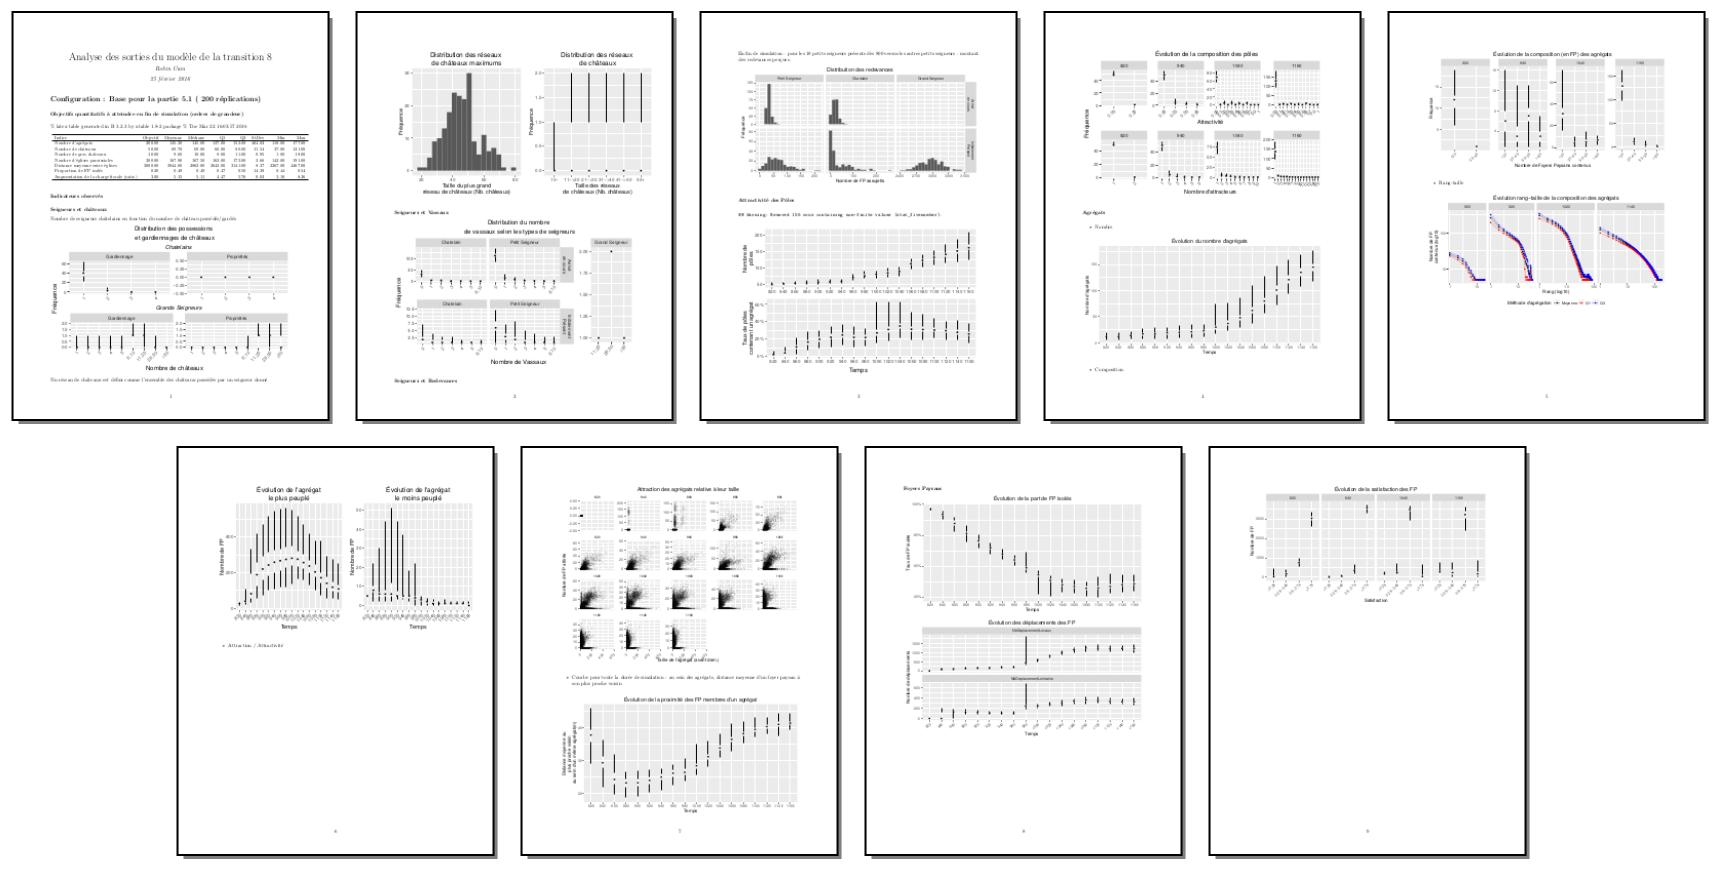
\includegraphics[width=\linewidth]{img/SimFeodal_Rapport_exemple.png}
		\caption{Un exemple de rapport automatique généré pour une expérimentation (étape 0) de SimFeodal. La version en taille réelle est reproduite en \hl{annexe X}.}
		\label{fig:simfeodal_rapport_mini}
	\end{figure}

\clearpage
	\paragraph{Structurer des rapports pour aller vers la reproductibilité des analyses}
	On a donc fait le choix de se baser sur des rapports automatisés et minimalistes, ne contenant que les indicateurs dans une forme structurée.
	Ce choix s'appuie sur des raisons multiples, qui ont toutes en commun une recherche de reproductibilité des résultats et des analyses menées.
	Une reproductibilité théorique (\hl{encore une ref au positionnement}), puisque les résultats de simulation doivent pouvoir être analysés et reproduits par des chercheurs potentiellement intéressés.
	Mais cette recherche de reproductibilité est aussi pratique, rendue aussi nécessaire par les méthodes de modélisation suivies.
	Tel qu'explicité auparavant (\cref{subsec:capter-replications,subsec:capter-experiences}), celles-ci s'appuient sur de nombreux allers-retours, ce qui requiert une capacité constante à reproduire et à affiner des résultats déjà observés.
	
	La quantité d'expériences requises pour arriver à un état satisfaisant du modèle est tributaire de ces allers-retours, et le nombre de rapports qu'il faut pouvoir produire est important.
	La fréquence de production de ces rapports est forte, et le modélisateur a alors tout intérêt à en fluidifier et accélérer le processus de création.
	
	Dans une telle situation, la création d'un rapport automatisé garantit une calcul et une production simplifié et rapide des indicateurs sur les nouvelles données.
	Cela permet un examen des sorties de simulation presque immédiatement après leur exécution.
	Cette automatisation permet aussi de mener une seconde évaluation -- après le pré-filtrage constitué par l'observation d'indicateurs en direct -- du bon déroulement \og interne \fg{}\footnote{
		Au sens de l'évaluation interne, c'est-à-dire du bon fonctionnement, exempt de \textit{bugs}, du modèle de simulation implémenté.
	}.
	Le caractère fixe d'un rapport automatisé se base ainsi sur une structure de données contraignante, par exemple constitués en \textit{n} fichiers dotés de plusieurs colonnes spécifiquement attendues.
	Les caractéristiques de ces données sont elles-mêmes contraignantes.
	Un rapport automatisé ne fonctionne, par exemple, qu'en présence d'un nombre pré-défini de réplications complètes.
	En l'absence d'un de ces critères dans des données en sortie de simulation, le rapport ne peut être généré et émet une erreur.
	Par exemple, si le nombre de réplications est plus faible qu'attendu, ou encore si tel attribut d'un agent a changé de type informatique, la création du rapport échoue.
	La présence ou non de cette erreur constitue donc un nouveau filtre de vérification de la validité du modèle.
	Cela permet, là encore, de détecter des simulations qui présenteraient des comportements incomplets ou aberrants en terme de production de données.

	Un autre intérêt majeur des rapports, déjà pointé en avantage des outils de type \textit{CLI} est leur adaptabilité.
	On a vu (\hl{chap. 3}) que les indicateurs à examiner sont nombreux et surtout, évolutifs, dans le sens où ces indicateurs ont fortement été modifiés, remplacés, affinés, au cours des étapes de paramétrage de SimFeodal.
	L'utilisation de rapports automatiques permet de minimiser le nombre de modifications à effectuer en cas de changements d'indicateurs.
	Le programme informatique qui génère les rapports s'appuie ainsi sur un code-source unique, générique aux simulations de chaque modèle.
	Lors d'un changement d'indicateurs, il suffit alors de modifier ce code-source en une seule place, et tous les appels à ce programme seront alors modifiés en conséquence.
	À partir de là, pour mettre à jour l'ensemble des rapports déjà produits, c'est-à-dire regroupant les indicateurs de chacune des expériences passées, il suffit de ré-exécuter la routine de production des rapports.
	
	Dans le cas de SimFeodal, caractérisé par de fréquents changements dans la forme et le calcul des indicateurs, cela a représenté un gain de temps et d'efficacité très conséquent.
	Par exemple, lors de certaines phases de paramétrage, on pouvait être amenés à faire évoluer le modèle quotidiennement et à tester, à cette même fréquence, plusieurs jeux de paramètres.
	Il fallait donc analyser les résultats de plusieurs expériences chaque jour, et régulièrement ajouter des indicateurs graphiques afin d'affiner l'évaluation.
	Ces indicateurs devaient aussi être ajoutés aux expériences des jours précédents, et au final, on re-générait parfois jusqu'à une plus d'une dizaine de rapports sur des cycles temporels courts de quelques jours.
		
	Par extension, cette même démarche d'automatisation, basée sur l'utilisation d'outils de type \textit{CLI}, devrait pouvoir s'appliquer à l'identique, avec les mêmes avantages, dans le cadre plus large de l'évaluation visuelle de modèles (\hl{ref chap 3, section 3.1.4}).

%	\begin{encadre}{Générer les rapports avec \texttt{R} et \texttt{knitr}}{technique-rapports-knitr}
%
%		\hl{Encadré sur les rapports automatiques, le \textit{\og litterate programming}\fg, le choix et le paramétrage de knitr + lien vers le code-source des rapports.}
%
%	\end{encadre}


	\paragraph{Dépasser les limites de la compatibilité d'ensemble}
	En réalité, la démarche de reproductibilité des rapports constitue plus un objectif théorique qu'un stade, \og reproductible\fg{} qu'il serait possible d'atteindre.
	Il s'agit ainsi plus de s'inscrire dans la voie de la reproductibilité que de chercher à parvenir à cet objectif largement inaccessible dans les faits.
	
	Comme explicité dans l'hl{encadré 3.2} sur l'incrémentalité des indicateurs, une limite forte empêche d'atteindre une reproductibilité absolue des analyses du comportement des différentes versions de SimFeodal.
	Les données générées par les différentes versions du modèle ne sont en effet pas systématiquement \og compatibles \fg{}.
	On entend par là qu'elles ne présentent pas toute exactement la même structure, à commencer par les variables enregistrées.
	Quand bien même il aurait été choisi dès le départ d'enregistrer le plus de sorties possibles, la reproductibilité de l'analyse échoue sur les données produites par le modèle et ses nombreuses versions : le modèle évolue, et avec lui, certaines variables apparaissent et d'autres deviennent caduques.
	La structure contraignante et précise des données nécessaires à la génération des rapports ne peut être entièrement satisfaite.
	La prise en compte de l'évolution du modèle demande une adaptation régulière -- mais aussi rare que possible -- des programmes qui génèrent ces rapports.
	
	On ne peut donc satisfaire globalement à un objectif de reproductibilité, mais il est toutefois possible de limiter la déviance à cette ambition.
	Pour cela, on peut agencer les différentes versions du modèles au sein de \og générations\fg{} de modèle, c'est-à-dire d'ensembles de versions présentant des attributs comparables et générant des données de même structure.
	Plutôt que d'adapter le code-source des rapports à chaque nouvelle version du modèle, ou encore de ne jamais l'adapter et donc d'être tributaire de la structure des toutes premières versions du modèle, cela constitue un choix intermédiaire qui permet de limiter le nombre de variantes de rapports.
	Cette approche suit les grandes lignes du développement logiciel général. Les itérations successives d'un logiciel sont constituées de versions \og majeures\fg{} -- les générations de modèles dans notre cas --, qui n'assurent pas nécessairement de compatibilité avec les versions majeures précédentes, et de versions \og mineures\fg{}, dans lesquelles la compatibilité est assurée\footnote{
		Par exemple, un fichier de dessin vectoriel créé avec le logiciel Adobe Illustrator 15.0 ne sera pas lu correctement avec une version 14.0.
		Ce fichier présentera toutefois un compatibilité parfaite avec les versions 15.1 à 15.\textit{n} du logiciel.
	}.
	
	Pour revenir aux rapports voués à l'évaluation d'un modèle, en inscrivant les différentes versions du modèle -- et des programmes générant les rapport correspondant -- dans des sous-ensemble de versions, les \og générations\fg{}, les différents rapports peuvent être considérés comme reproductibles et automatiques au sein de ces générations.
	Pour SimFeodal, cela implique d'organiser les différentes versions du modèle -- résultant des étapes de paramétrage, \hl{cf. chap4} -- au sein de grandes générations, à chaque changements structurels des mécanismes ou données produites par le modèle.
	
	\hl{Ajouter un schéma avec les générations, versions et sous-versions}
	
	\paragraph{Les rapports, des instruments suffisants ?}
	
	A l'issue de la conception et de l'implémentation de ces rapports automatiques, on dispose donc, pour chaque expérience, d'un document aisément partageable et lisible.
	Ces documents s'enrichissent, au fur et à mesure des générations de modèles, de nouveaux indicateurs, et sont comparables au sein de ces générations.
	Cela pourrait constituer la dernière étape de la création d'outils d'évaluation d'un modèle, dans la limite d'un nombre de versions ou de génération de modèles assez restreint.
	
	SimFeodal, comme c'est souvent le cas dans les modèles à base d'agent, a toutefois été caractérisé par une forte quantité d'allers-retours entre le modèle et ses résultats, entraînant à chaque fois de nouvelles expérimentations (cf. \cref{sec:sorties-simfeodal}). 
	
	On a vu que la manipulation d'un grand nombre d'indicateurs, même pour une quantité restreinte d'expériences, disqualifiait l'usage de fichiers individuels et poussait à l'usage de rapports structurés.
	Avec un grand nombre d'expériences, les mêmes limites apparaissent pour les rapports : la masse d'expériences rend partiellement caduque l'utilisation unique des rapports automatiques.
	Il est en effet aisé de comparer, sur un même écran d'ordinateur, deux ou trois rapports, mais dès lors qu'il faut en comparer un plus grand nombre, la manipulation conjointe des rapports devient complexe, tout autant que d'avoir une vision globale des résultats principaux de chaque expérience.

\clearpage
	\subsection{Organiser les rapports : Dashboards}\label{subsec:dashboards}

	Pour être en mesure de comparer de nombreux éléments, il est nécessaire de passer d'une exploration linéaire, fondée sur le visualisation successive de chacun des indicateurs, à une exploration globale et interactive.
	En pratique, plutôt que de faire défiler visuellement les nombreuses pages d'indicateurs, mieux vaut une interface présentant les points clefs de l'évaluation et qui permette d'entrer dans le détail de chacun des indicateurs dans un second temps, sur demande.
	Comme le résume le \og mantra\fg{} de l'analyse visuelle (\og \textit{Visual information-seeking mantra}\fg{}) de \citeauteur{shneiderman1996eyes} :
\begin{quote}
	\centering
	\noindent\og Overview first, zoom and filter, then details on demand\fg{}\\
	\mbox{}~ \hfill \cite[\ppno~2]{shneiderman1996eyes}
\end{quote}
	

	\subsubsection{Les \textit{dashboards}}

	Cette logique, assez universelle désormais, est celle qui préside à la création des nombreux \og tableaux de bord \fg{}, ou \og \textit{dashboards} \fg{} que l'ont voit émerger depuis la fin des années 1990.
	Rob Kitchin et ses co-auteurs définissent ainsi les \textit{dashboards}, en s'appuyant sur les travaux de Few notamment :

	\begin{quotation}
		\og For Few [\autocite[p.34]{few_information_2006}] a ‘dashboard is
		a visual display of the most important information needed to achieve one or more objectives; consolidated and arranged on a single screen so the information can be monitored at a glance’.
		Just as a car dashboard provides critical information needed to operate the vehicle at a glance, indicator dashboards provide key information for running companies or cities (\st{Dubriwny \& Rivard, 2004})[\autocite{rivard_are_2004}].\fg{}\\
		\mbox{}~ \hfill \cite[p. 11]{kitchin_knowing_2015}
	\end{quotation}

	Très répandus dans le monde de l'informatique décisionnelle (\textit{Business Intelligence, BI}), ces outils permettent d'explorer des données d'entreprises, par exemple des résultats financiers.
	Pour ce faire, ils mettent en avant, dans une interface unique, des indicateurs clés (\textit{Key Performance Indicators, KPI}), qu'il est ensuite possible de filtrer et d'affiner, par exemple par sélection de différents intervalles temporels.

	Les \textit{KPI} jouent le rôle d'indicateurs synthétiques, c'est-à-dire qu'ils s'adressent à des gestionnaires, par exemple des \textit{managers}, qui ont une expertise importante sur les résultats produits.
	Les utilisateurs des \textit{dashboards} ne sont donc pas des analystes, à même d'explorer eux-mêmes les données mobilisées, mais plutôt des thématiciens qui se fondent sur les indicateurs présentés pour prendre des décisions.

	La dichotomie \og analyste/décisionnaire\fg{} s'exprime aussi dans le domaine de la recherche, et notamment dans la recherche en géographie urbaine à visée applicative.
	Avec l'avènement des données massives et de leur prise en compte pour la gestion des villes (\textit{smart cities}), les géographes se sont aussi penchés sur des outils de ce type.
	En résulte une utilisation de plus en plus fréquente de \textit{dashboards} en géographie urbaine (\og \textit{city-dashboards}\fg{}, \cite{roumpani_creating_2013, kitchin_knowing_2015, batty_perspective_2015}).

	Le parallèle avec le monde de l'informatique décisionnelle est en effet présent dans les types d'utilisateurs et de producteurs de ces outils.
	Il s'agit de mettre à disposition d'experts thématiques (les décideurs publiques) des indicateurs clés, issus de calculs parfois complexes.
	Cela afin de leur permettre d'évaluer une situation donnée et de prendre les décisions politiques adéquates.

	Le constat ayant mené à l'apparition des premiers \textit{dashboards}, tant en informatique décisionnelle qu'en géographie urbaine, est identique.
	Les informations nécessaires à l'évaluation d'une situation (financière, relative aux politiques publiques\ldots) sont de plus en plus nombreuses et hétérogènes.
	Les indicateurs permettant de mener ces évaluations, pensés pour les décideurs qui en feront usage (\textit{managers}, acteurs publiques\ldots), se démultiplient et se diversifient aussi par conséquence.

	Inspiré autant par l'usage \textit{BI} que par l'usage géographique, nous considérons que ces outils peuvent se révéler utiles dans l'évaluation de modèles de simulations complexes.
	Les enjeux sont en effet les mêmes : permettre à des thématiciens de comprendre et d'évaluer les sorties d'un modèle, à l'aide d'indicateurs nombreux et complexes présentés de manière transparente relativement à cette complexité.

	Ce positionnement méthodologique s'inscrit pleinement dans la démarche de co-construction interdisciplinaire de SimFeodal.
	On y retrouve ainsi la même logique qui anime les dashboards : une évaluation menée par des thématiciens qui s'appuient pour cela sur des indicateurs clefs (\hl{ref. aux indicateurs les plus importants dans le chap 3}) et précisent leur analyse à l'aide d'indicateurs secondaires présentés sous forme d'un panel varié de visualisations.
	Nous avons donc choisi de ré-organiser les rapports initialement produits pour leur donner une forme plus adaptée à ces enjeux, sous forme de \textit{dashboards}.

	\subsubsection{SimVADB}\label{subsubsec:simvadb}

	Les \textit{dashboards} font souvent usages de représentations graphiques très métaphoriques des tableaux de bords automobiles.
	On y retrouve fréquemment une forte mise en valeur d'indicateurs numériques simples au travers de représentations \og skeuomorphes\fg{}, c'est-à-dire qui reprennent l'apparence physique des objets symbolisés.
	On retrouve communément, par exemple, des indicateurs représentés sous forme de jauges (\textit{gauge charts}), de thermomètres (\textit{thermometer charts}), ou encore de voyants d'alerte et autres témoins lumineux (\cref{fig:skeuomorphism})).
	
	\begin{figure}[H]
		\centering
		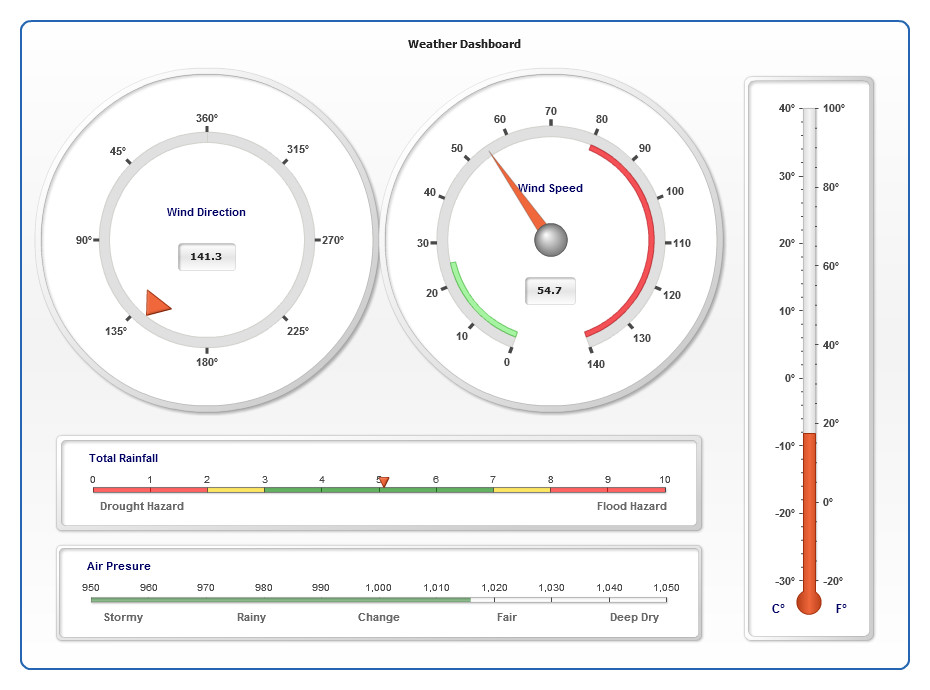
\includegraphics[width=.8\linewidth]{img/skeuomorphism.jpg}
		\caption{Un exemple de représentations visuelles courantes dans les \textit{dashboards}. Tiré de \textcite{pandre_charts_2011}}
		\label{fig:skeuomorphism}
	\end{figure}
	
	
	Pour SimFeodal, les indicateurs étant assez fortement conçus et structurés (\hl{chap. 3}), nous n'avons pas ressenti le besoin de faire appel à ce type de représentation.
	Nous avons donc emprunté aux \textit{dashboards} la logique d'organisation visuelle des indicateurs plutôt que les modes de visualisation en eux-mêmes.
	Pour faciliter la transition pour l'utilisateur, on cherchait ainsi à produire un \textit{dashboard} au plus proche, visuellement, des rapports automatiques qui les précédaient.

	On a pour cela développé un \textit{dashboard} adapté à SimFeodal, nommé SimVADB\footnote{
	\textbf{S}imulation \textbf{V}isual \textbf{A}nalysis \textbf{D}ash\textbf{B}oard.\\
	Cette application a rapidement été remplacée par l'itération suivante (SimEDB, voir \cref{subsec:explo-interactive}), et n'a donc dans les faits jamais été complètement finalisée. On en trouve une trace, fonctionnelle mais incomplète (les versions ultérieures n'ont pas été enregistrées dans l'outil de versionnement), dans ce dépôt logiciel :
	\href{https://github.com/RCura/SimEDB/tree/2cd22c7ccfbcf31f4a09550c2396932c46ef2622}{https://github.com/RCura/SimEDB/tree/2cd22c7c}
	}.
	Dans un premier temps, on souhaitait simplement ré-organiser le code-source produisant les rapports automatiques, afin de convertir ces rapports en \textit{dashboards}.
	Cela a été effectué au moyen d'outils permettant de générer des applications en ligne, sans changer de langage de programmation.
	Dans ce cas, on s'est appuyé sur la librairie logicielle \textsf{Flexdashboard} \autocite{iannone_flexdashboard_2018}.
	
	Le passage du rapport automatique au \textit{dashboard} illustre l'un des grands intérêts des outils de type \textit{CLI} : dans le cas de SimVADB, il a suffit de ré-organiser le code, sans modifier à aucun moment les fonctions de calcul et de création des indicateurs de sortie de simulation.
	Les codes \ref{lst:code-rapport} et \ref{lst:code-dashboard} illustrent la facilité de cette modification.
	Il s'agit véritablement de placer les différentes fonctions dans des blocs graphiques.
	Ces modifications minimes augmentent toutefois considérablement la convivialité et la facilité de l'analyse de résultats de sortie d'un modèle.
\clearpage

\lstset{frame=shadowbox, tabsize=2}
\noindent\begin{minipage}[t]{.44\textwidth}
{\footnotesize
	\begin{lstlisting}[caption={Pseudo-code du rapport automatique.},frame=tlrb, captionpos=b, label = {lst:code-rapport}]
# Agent de type A
	afficher('Agent de type A')
	
	print('Indicateur 1')
	calcul_indicateur_1 {...}
	affichage_indicateur_1 {...}
	
	afficher('Indicateur 2')
	calcul_indicateur_2 {...}
	affichage_indicateur_2 {...}
# Agent de type B
	afficher('Agent de type B')
	[...]
	\end{lstlisting}
}
\end{minipage}\hfill
\begin{minipage}[t]{.53\textwidth}
{\footnotesize
	\begin{lstlisting}[caption={Pseudo-code du dashboard.},frame=tlrb, captionpos=b, label = {lst:code-dashboard}]
onglet{titre = 'Agent de type A',
	sous_onglet{titre = 'Indicateur 1',
		calcul_indicateur_1 {...}
		affichage_indicateur_1 {...}
	},
	sous_onglet{titre = 'Indicateur 2',
		calcul_indicateur_2 {...}
		affichage_indicateur_2 {...}
	}
},
onglet{titre = 'Agent de type B',
	[...]
}
	\end{lstlisting}
}
\end{minipage}
	
	Comme dans l'exemple de code, on a préféré organiser les indicateurs au seins d'onglets plutôt que de les présenter dans des pages successives.
	Les onglets de premier niveau représentaient les types d'agent, et des onglets de second niveau permettaient de visualiser l'ensemble des indicateurs associés à ces agents (\cref{fig:mockup_simvadb}).

\begin{figure}[H]
	\centering
	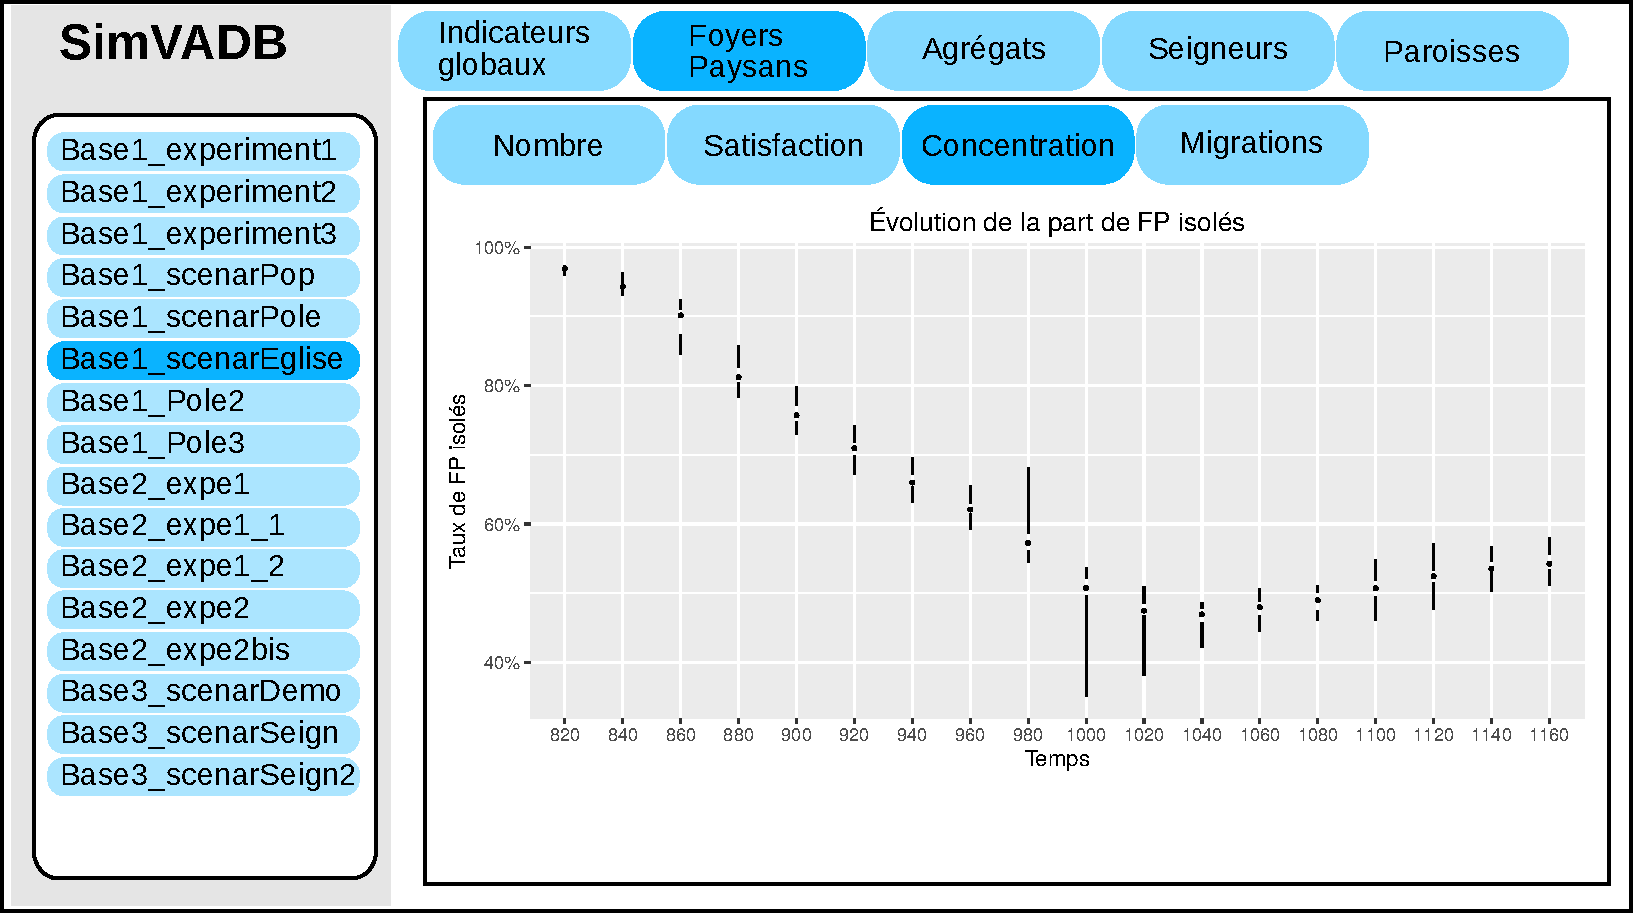
\includegraphics[width=\linewidth]{img/simvadb_mockup.pdf}
	\caption{Un \textit{mock-up} de la première interface de SimVADB, un \textit{dashboard} dédié à la visualisation des indicateurs de sorties de simulation de SimFeodal.}
	\label{fig:mockup_simvadb}
\end{figure}

	Au niveau de l'interface utilisateur, SimVADB permettait de choisir, via un menu de sélection (partie de gauche dans la \cref{fig:mockup_simvadb}), les expériences passées dont on voulait visualiser les indicateurs de sortie (les deux niveaux d'onglets de la partie de droite).

	
	\paragraph{Les limites du \textit{dashboard}}
	Avec la multiplication des valeurs de paramètres testées, il est devenu plus efficace de regrouper les expériences au sein d'expérimentations.
	Celles-ci voient varier plusieurs paramètres, potentiellement avec de multiples valeurs de paramètres pour chacun.
	Elles constituent donc un ensemble d'expériences qui partagent des mécanismes et un jeu de paramètre par défaut communs.

	Avec le mode de sélection choisi dans SimVADB, basé sur le nom des expériences, il devenait plus difficile de sélectionner rapidement des ensembles d'expériences membres d'une même phase d'expérimentation.
	En effet, et comme illustré dans la \cref{fig:mockup_simvadb}, les noms d'expériences tendent à s'allonger, et avec leur masse augmentant, il est peu commode d'avoir à parcourir tout un long menu de sélection pour trouver les expériences souhaitées.
	De plus, malgré des tentatives de nommage régulières et explicites, la multiplication des expériences et expérimentations implique aussi une certaine confusion dans les types de mécanismes et valeurs de paramètres associés.
	Sans table de correspondance complète entre les noms des expériences et leurs valeurs de paramètres, il devenait impraticable de retrouver les différentes expériences mettant en avant, par exemple, des attractivités fortes par les pôles, une plus forte hiérarchisation des attracteurs ou encore des migrations lointaines facilitées.
	Le choix méthodologique d'interaction avec la plate-forme d'affichage des indicateurs, basé sur une sélection des expériences depuis leur nom, s'est donc révélé inadapté à la sélection et à l'exploration des sorties de SimFeodal.
	
	
	Au delà du soucis du mode d'interaction, qui aurait pu être amélioré, un autre problème apparaissait.
	Pour évaluer visuellement différentes configurations du modèle, on ne pouvait se contenter d'un simple affichage des données, au sein d'un outil de type présentoir interactif tel que SimVADB.
	Comme dit dans \hl{le chapitre 4}, le paramétrage de SimFeodal a ainsi reposé sur de nombreuses étapes d'évaluation des différentes version du modèle.
	L'approche d'analyse principale était donc la comparaison, point par point, entre les résultats des indicateurs de sortie de simulation des versions successives de SimFeodal.
	Un outil de présentation dynamique de résultats de sorties de simulations est certes plus adapté qu'un rapport statique, mais il ne constitue pas pour autant un outil adapté à la comparaison.
	S'il suffit pour de la restitution, par exemple dans le cadre du rapport systématique des résultats de SimFeodal, on ne peut s'appuyer uniquement sur une succession d'évaluations visuelles pour appréhender l'étendue des changements apportées par une modification des valeurs de paramètres.

	\subsection{Interagir avec les rapports : exploration interactive}\label{subsec:explo-interactive}

	Face à la démultiplication des expérimentations, consécutive aux nombreuses étapes de paramétrage de SimFeodal (\hl{cf. chap 4}), il a fallu repenser la plate-forme d'évaluation des résultats.
	Pour cela, considérant que les simulations ne pouvaient être aisément appréhendées et sélectionnées par leur nom, numéro d'étape ou de version, il a été décidé d'adopter une posture plus proche de l'exploration du modèle en elle-même.
	C'est-à-dire de ne pas caractériser les simulations par un identifiant quelconque, mais plutôt par leur spécificité intrinsèque, c'est-à-dire la combinaison de valeurs de paramètres qui les rendent uniques.
	Ce faisant, au sein de la plate-forme d'exploration SimVADB, l'enjeu devenait plutôt la compréhension des effets des valeurs de paramètres sur les indicateurs que l'évaluation d'une simulation en particulier.
	Il fallait passer du descriptif, quelle qu'en soit la méthode, à du comparatif.
	
	Du point de vue de l'interface utilisateur, cela implique que la sélection ne se fasse plus par un unique critère (le nom de la simulation), mais au contraire sur du multi-critère.
	Par une succession de sélections, chaque paramètre pouvait constituer un nouveau filtre dans lequel on avait à choisir les valeurs à interroger (voir la \cref{fig:schema_parcoords} \textbf{(E)} de l'\cref{enc:parcoords}).

	La quantité de paramètres en entrée était importante et pouvait dès lors donner lieu à un mode de sélection complexe et fastidieux -- définir une par une les valeurs voulues pour chacun des 45 paramètres --.
	Nous avons choisi encore une fois de nous appuyer sur l'aspect visuel afin de permettre aux utilisateurs de SimVADB de choisir la ou les expérimentations à analyser.
	
	
	\paragraph{Visualiser avec des coordonnées parallèles }

	Pour cela, on a choisi de représenter les combinaisons de paramètres dans un graphique en \og coordonnées parallèles \fg{} (\textit{parallel coordinates}, d'après \cite{inselberg_parallel_1987}, voir \cite{few_multivariate_2006} par exemple pour une description plus succincte, illustrée et pratique).
	Ce type de graphique est en effet extrêmement pertinent pour représenter une information multi-dimensionnelle en ce qu'il permet de détecter graphiquement des \textit{clusters} d'individus statistiques\footnote{
		Ici, chaque expérience est un individu statistique.
		Il est caractérisé par un ensemble de variables, les différents paramètres, et les modalités de ces variables que cet individu emprunte (les valeurs de paramètres).
		Quand le nombre d'individus est important, les différentes \og courbes\fg{}, qui correspondent au profil des individus sur le graphique en coordonnées parallèles, peuvent se superposer et montrer des tendances similaires.
		Avec ce type de représentation, il est facile de visualiser les grandes classes d'individus constituées par ces \og tendances\fg{}, et donc de constater des distinctions entre les individus (les expériences) de manière visuelle.
	} \autocite[2]{heinrich_state_2013}, c'est-à-dire de faire ressortir visuellement les expériences dont les valeurs de paramètre sont proches.
	Notons bien que l'on parle ici des valeurs de paramètres, c'est-à-dire des conditions des expériences, et non des indicateurs de sortie.
	L'approche va ainsi des paramètres aux résultats : depuis des valeurs de paramètres choisies, on analyse la diversité des résultats.
%	L'approche inverse, souvent menée en simulation agent (\hl{ref à chap 3, exploration automatique}}), pourrait mener une classification des résultats de sortie pour reporter cette classification sur les valeurs de paramètres.

	
	\paragraph{Interagir avec des coordonnées parallèles}
	De plus, en matière d'interaction, on utilise fréquemment les graphiques en coordonnées parallèles en vue de filtrage.
	Cette opération est le plus souvent menée par des actions de \textit{brushing} (\og brossage\fg{}), c'est-à-dire de sélection graphique d'une zone en dessinant son étendue à la souris (voir \cref{enc:parcoords}).
	Ce type de sélection se révèle en effet souvent plus efficace et intuitive qu'une sélection textuelle plus systématique :
	
	\begin{quotation}\vspace{-0.5cm}
		\og Filtering is an operation that removes signals from its input. A filter reduces the number of lines to be rendered. In this sense, dynamic querying [...] is a filter, if implemented with brushing [...], which reduces clutter by putting the filtered lines in focus using some highlighting mechanism. Combining simple brushes using logical operators [...] further allows the user to formulate rather complex queries that might even achieve faster and more accurate results using parallel coordinates than using a Structured Query Language (SQL) [...].\fg{}\\
		\mbox{}~ \hfill \cite[p. 13]{heinrich_state_2013}
	\end{quotation}
	
	\begin{encadre}{Construction et utilisation interactive d'un graphique en coordonnées parallèles}{parcoords}

	La \cref{fig:schema_parcoords} illustre les étapes successives de construction d'un graphique en coordonnées parallèles, depuis le tableau statistique (\textbf{A}) jusqu'au graphique final (\textbf{D}).
	
	Pour cela, on projette les valeurs des variables sur des axes représentant chacune des variables (\textbf{B}).
	En normalisant la taille de ces axes et en les plaçant en parallèle (\textbf{C}), on peut alors tracer les \og profils\fg{} des variables en reliant les positions de chacun des individus statistiques sur chacun des axes (\textbf{D}).
	
	La seconde partie de la figure représente le mode d'interaction par \textit{brushing} : on \og brosse\fg{} sur chaque axe une sélection de valeurs à conserver (\textbf{E}).
	La sélection graphique est convertie en intervalles numériques et formalisée sous une forme classique (\textbf{F}) qui permet de filtrer les données sous-jacentes.
	Au final, cette opération renvoie le seul individu statistique répondant aux deux sélections graphiques (\textbf{G}).
	
	\begin{figure}[H]
	\centering
	\captionsetup{width=\linewidth}
	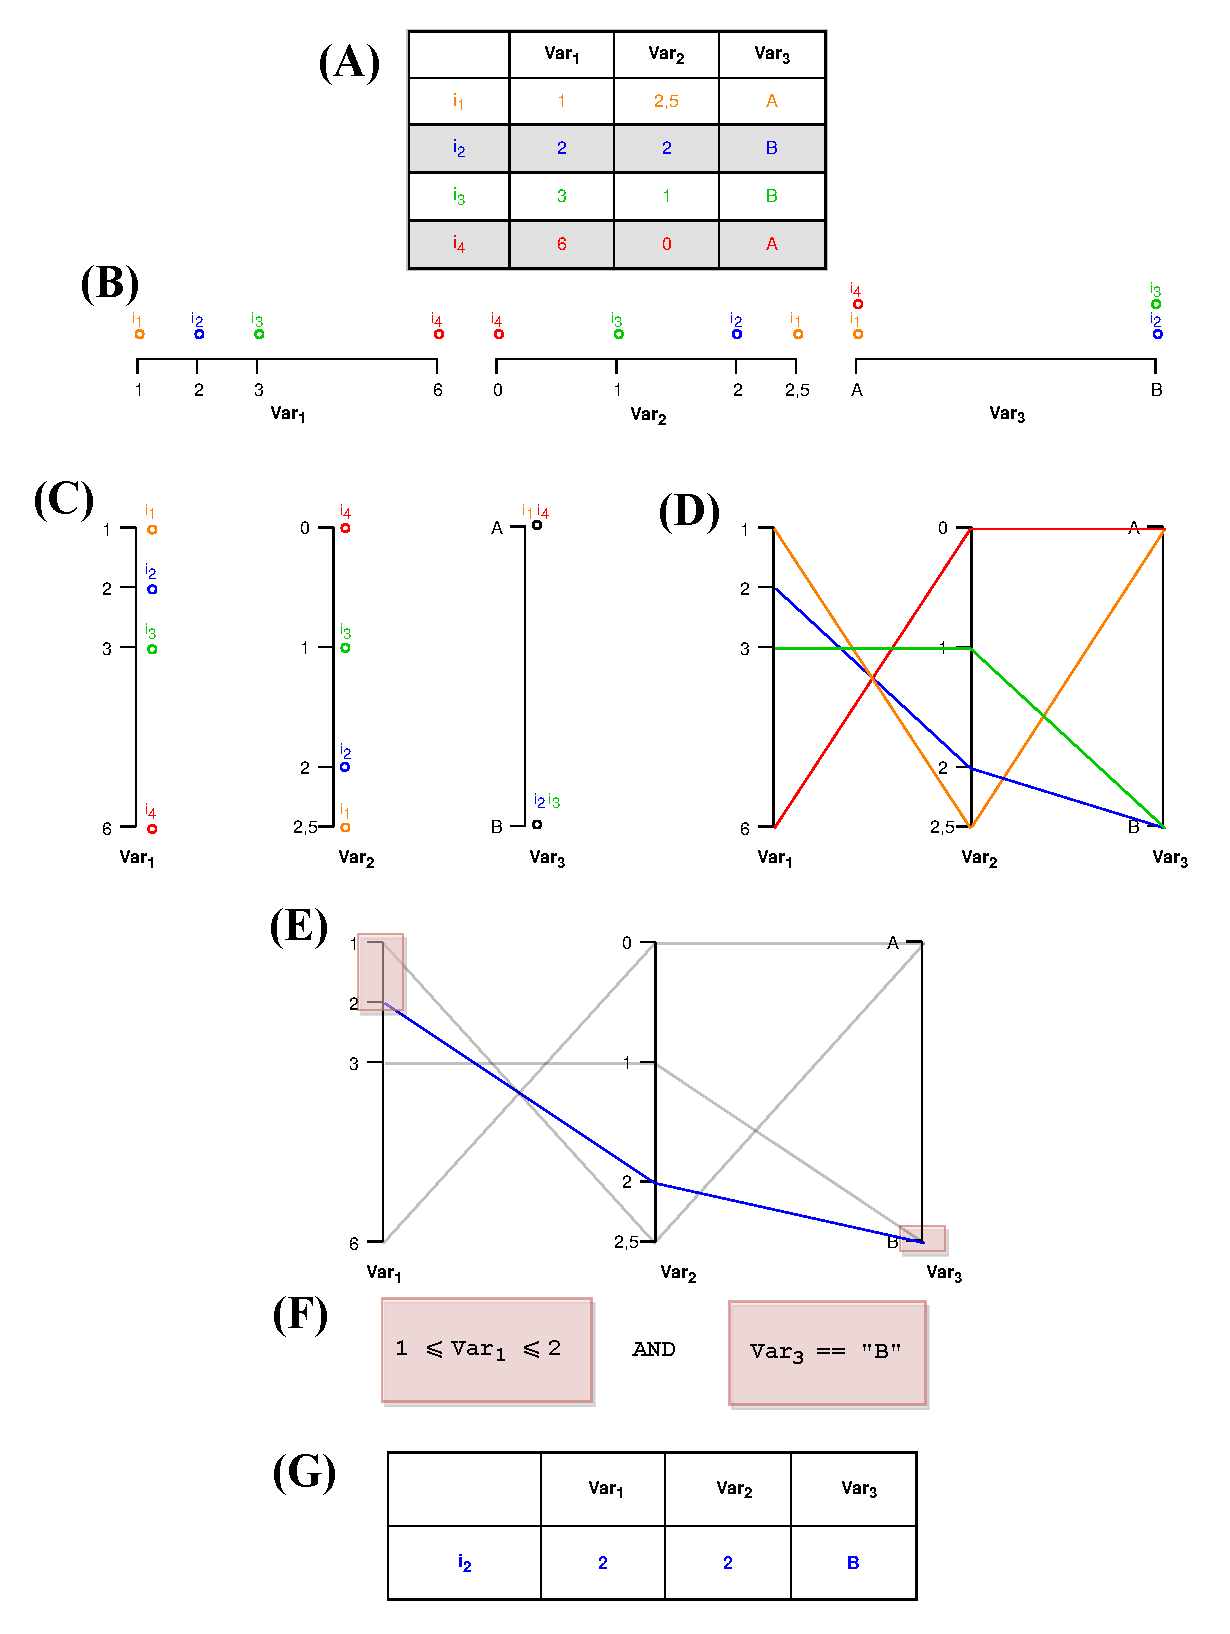
\includegraphics[width=.94\linewidth]{img/ParCoords_Brush.pdf}
	\caption{Construction d'un graphique en coordonnées parallèles et sélection interactive.\vspace{.1cm}}
	\label{fig:schema_parcoords}
	\end{figure}

	\end{encadre}


	Cette utilisation est aussi courante en géographie quantitative, et on la retrouve par exemple chez l'un des représentants de l'analyse spatiale des années 1990, Stewart Fotheringham.
	Cet auteur indique même l'usage du graphique en coordonnées parallèles en tant que filtre pour identifier des informations dans une autre dimension, spatiale ici : \og the data being displayed in parallel coordinates can be linked to a map and then brushed to highlight the locations of interesting lines displayed in \textit{m}-space on the parallel co-ordinates.\fg{} \autocite{fotheringham_trends_1999}.

	Appliqué aux données de SimFeodal, cette interface (\cref{fig:simvadb_dashboard}) se révèle particulièrement efficace pour sélectionner les configurations de paramètres à explorer.
	Ainsi, en \og brossant \fg{} quelques filtres manuellement (\cref{fig:simvadb_dashboard} - \textbf{A}), on arrive rapidement à isoler une expérience spécifique.

	\begin{figure}[H]
		\captionsetup{width=\linewidth}
		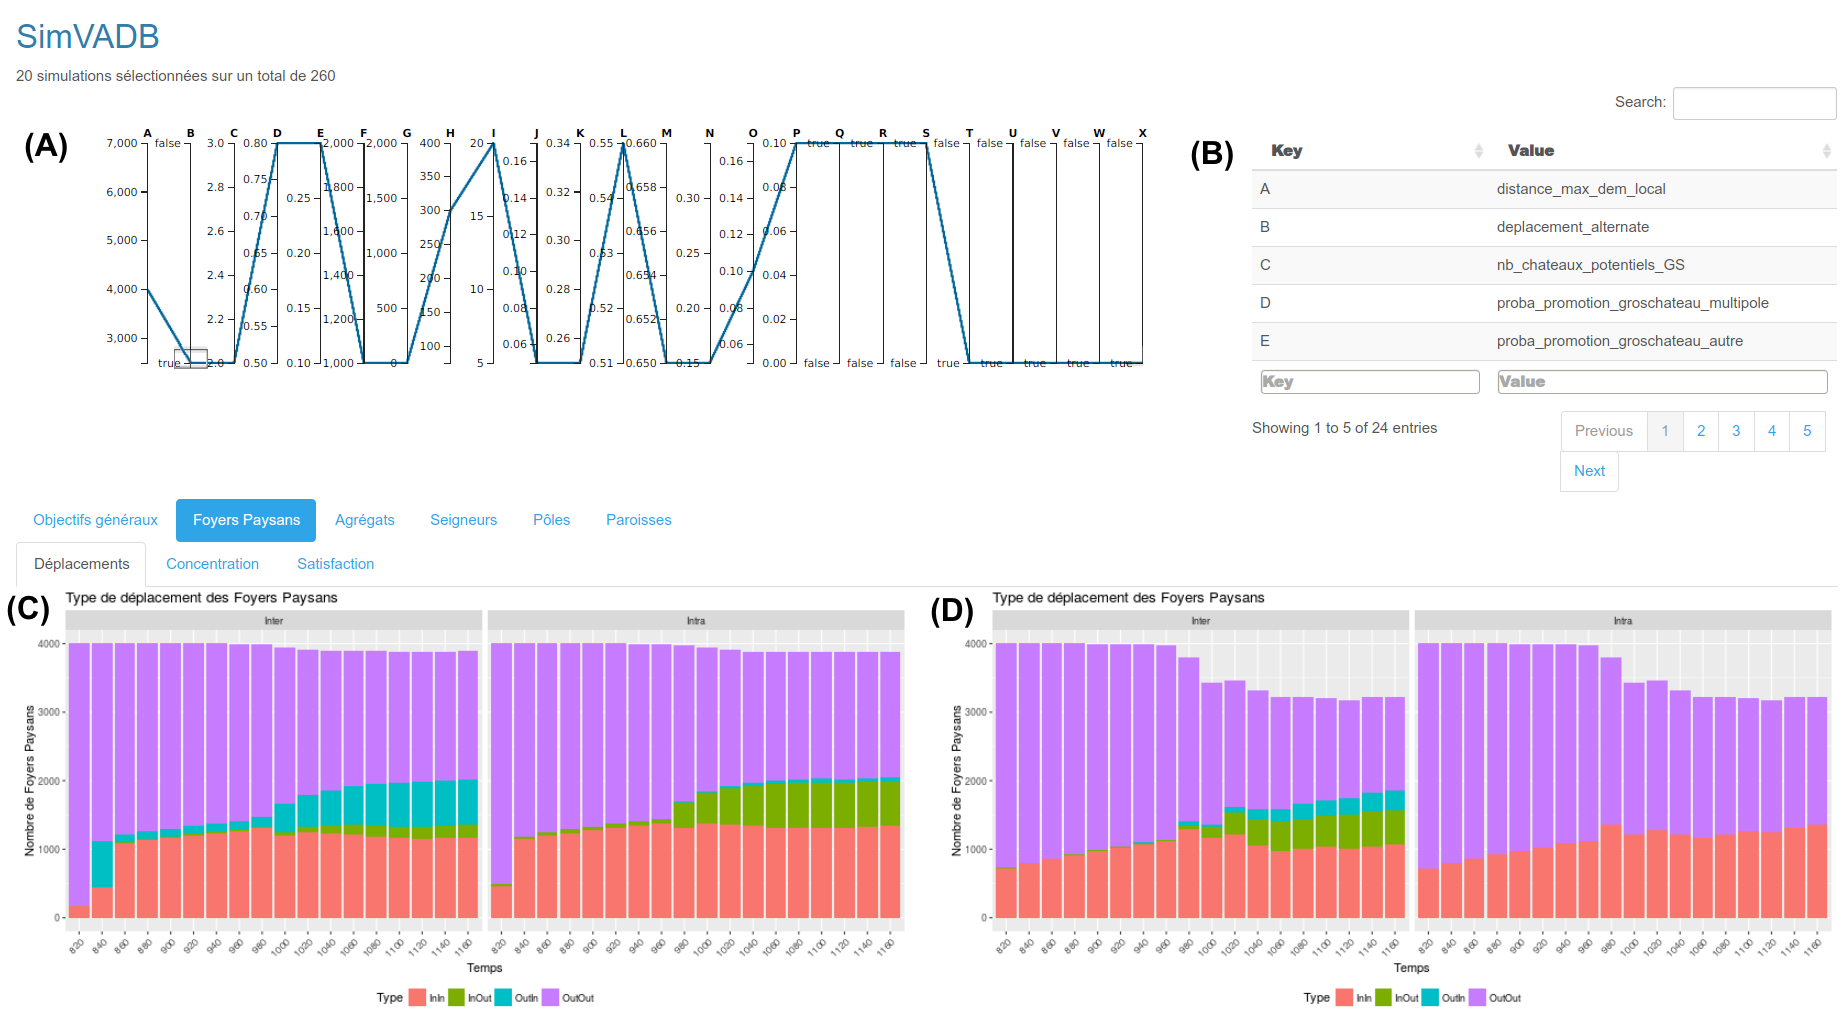
\includegraphics[width=\linewidth]{img/SimVADB_Dashboard2_annote_retouche.png}
		\caption{SimVADB (Simulation Visual Analysis DashBoard), un \textit{dashboard} d'exploration visuelle des indicateurs de sortie de simulation de SimFeodal.\\
		La sélection des simulations à explorer se fait dans le graphique en coordonnées parallèles (\textbf{A}), en \og brossant\fg{} des filtres graphiques sur les \og dimensions\fg{} du graphique, dimensions dont les intitulés sont explicités dans le tableau \textbf{B}.
		Les graphiques \textbf{C} et \textbf{D} indiquent l'évolution des types de déplacements des foyers paysans au cours des simulations.\\
		- Le graphique \textbf{C} représente, pour cet indicateur, une moyenne de l'ensemble des simulations intégrées dans la base de données (260 ici), recouvrant donc plusieurs valeurs de paramètres.\\
		- Le graphique \textbf{D} représente cet indicateur calculé depuis un sous-ensemble de 20 simulations (donc une expérience composée de 20 réplications), pour lesquelles le paramètre \og \textsf{B} \fg{} (\textsf{deplacement\_alternate}) vaut \textsf{true}.}
		\label{fig:simvadb_dashboard}
	\end{figure}

	Afin de permettre aux utilisateurs de remarquer les particularités des simulations explorées, nous avons choisi de mettre en emphase les différences entre la tendance générale des indicateurs, en calculant des moyennes de l'ensemble des simulations (\cref{fig:simvadb_dashboard} - \textbf{C}), et les valeurs spécifiques des indicateurs de l'expérience choisie (\cref{fig:simvadb_dashboard} - \textbf{D}).
	Cela permet, visuellement, d'être en mesure d'évaluer les sorties de simulation d'une expérience tout en ayant un référentiel visible.
	Les différentes expériences produisent des résultats sensiblement similaires\footnote{
		Si chaque expérience, et chaque réplication, produisent des résultats uniques, le choix d'une évaluation par des indicateurs visuels peut prêter à confusion si l'on n'a pas de repère précis.
		Les critères attendus, présentés dans \hl{le chapitre 3} sont ainsi assez précis pour départager une simulation très éloignée des attentes et une autre simulation plus conforme.
		Pour autant, par exemple quand les valeurs de paramètres varient faiblement, les résultats produits peuvent être assez similaires dans les grandes tendances qu'ils font ressortir.
	}, et on ne peut alors plus les comprendre sans les confronter à d'autres résultats similaires.
	Le choix d'une agrégation de l'ensemble des simulations effectuées est discutable, en ce qu'on aurait par exemple pu plutôt isoler des simulations \og de référence \fg{} afin de diminuer l'effet \og d'aplatissement \fg{} engendré par l'agrégation de résultats nombreux et hétérogènes.
	Toutefois, la variabilité des résultats étant encore assez restreinte, au moment de la création et de l'utilisation de SimVADB, ce référentiel agrégé permettait déjà une compréhension plus fine des sorties de simulations, en particulier dans l'analyse de l'impact de variations fines de valeurs de paramètres.

	\subsection{Explorer en comparant : SimEDB}\label{subsec:explorer-simedb}

	Après un travail de paramétrage grossier qui permet de stabiliser les mécanismes, il est souvent nécessaire de passer à une phase plus fine.
	On vise à ce moment à mieux calibrer un modèle à l'aide de variations de valeurs de paramètres de granularité inférieures.
	En vue d'évaluer les simulations, et donc de les différencier les unes des autres à l'aune des indicateurs générés, la comparaison d'une expérience spécifique avec un référentiel constitué de toutes les expériences précédentes ne permet plus de mener ce travail de comparaison fine.
	Les variations entre simulations sont trop fines pour être distinguables les unes des autres par le biais d'une comparaison avec un référentiel unique\footnote{
	On peut prendre l'exemple de SimFeodal.
	En faisant varier le nombre de foyers paysans de $4000$ à $4200$ ($5\%$ de variation), les résultats du modèle changent peu : de faibles variations de valeurs de paramètres entraînent le plus souvent de faibles variations dans les indicateurs de sorties observés.
	On peut de plus noter que les répercussions d'un changement de valeur de paramètre peuvent être très différentes de l'ordre de grandeur de ce changement de valeur.
	Cela s'explique par la non-linéarité de l'influence des paramètres.
	Dans l'exemple pris, pour ces $5\%$ de variation dans le nombre de foyers paysans, la majorité des indicateurs variera ainsi de moins de $1\%$.
	}.
	Cela s'entend quelque soit la manière dont ce référentiel est constitué, qu'il résulte d'une agrégation de simulations ou encore d'une version \og de base\fg{} du modèle (par exemple, dans le cas de SimFeodal, les versions principales identifiées dans le \hl{chapitre 4}).
	

	Pour pouvoir correctement évaluer les apports d'un nouveau jeu de valeurs de paramètres, et donc, dans une démarche itérative, pouvoir différencier deux expériences successives, il est nécessaire d'être en mesure de comparer directement les expériences les unes avec les autres, ou encore avec un référentiel facilement ajustable.
	On peut énumérer les quelques exemples de cas de figure suivants :
	\begin{itemize}
		\item Comparaison entre une expérience spécifique et une autre expérience spécifique de même \og importance\fg{}.
		Par exemple, comparer deux expériences qui font varier légèrement différement une valeur de paramètre.
		\item Comparaison entre une expérience spécifique et une autre expérience spécifique d'\og importance\fg{} différente.
		Cette différence de niveau peut être constituée par exemple par une version \og de base\fg{} que l'on comparerait à une variante de celle-ci.
		\item Comparaison entre deux expérimentations, par l'agrégation de leurs résultats.
		Si l'on a mené des expérimentations faisant varier de manière systématique deux paramètres différents, il peut être intéressant de les comparer en bloc, c'est-à-dire par exemple en prenant les moyennes de chacune des expériences composant ces expérimentations.
	\end{itemize}
	
	Ce faisant, on fait en fait varier la notion de \og simulation de référence\fg{}, qui peut alors revêtir plusieurs formes.
	Pour cela, il n'est plus possible de mener une comparaison visuelle entre un référentiel commun et une expérience spécifique, mais bien de baser l'évaluation sur la comparaison entre deux ensembles spécifiques qui doivent pouvoir être spécifiés.
	D'un point de vue méthodologique, cela requiert de pouvoir afficher conjointement les indicateurs de sorties de deux expériences (ou ensembles d'expériences).
	Cela implique aussi de laisser à l'utilisateur la responsabilité d'un choix supplémentaire puisqu'il faut désormais effectuer deux sélections : une pour chacun des points de comparaison.
	La sélection d'une expérience via l'usage de \textit{brushing} sur un graphique en coordonnées parallèles des valeurs de paramètres ayant montré son efficacité, il a été choisi d'étendre ce principe d'interactivité au choix du référentiel.
	
	Dans cette version remaniée de la plate-forme d'exploration (voir \cref{fig:simedb_villages}), renommée SimEDB\label{par:introduction-nom-simedb} (\textbf{Sim}Feodal \textbf{E}xploration \textbf{D}ash\textbf{B}oard)\footnote{
		\label{ftn:origine-simedb}
		La plate-forme d'exploration SimVADB (SimFeodal Visual Analysis Dashboard) a été renommée SimEDB ([...] Exploration Dashboard) par soucis de simplicité, le terme \og Exploration\fg{} nous semblant plus compréhensible et explicite que celui de Visual Analysis.
		Ce nom apporte de plus une cohérence sémantique entre plusieurs productions de l'auteur -- TimeLineEDB - \autocite{cura_timelineedb_2017}; RoadTrafficEDB et CitiBikeEDB - \autocite{cura_making_2017}.
		Cela inscrit cette plate-forme d'exploration de données issues de simulation dans une \og famille \fg{} d'outils d'exploration de données spatio-temporelles.
	}, l'accent est mis sur la comparaison de deux ensembles de résultats, chacun répondant à une sélection propre.
	L'utilisateur doit ainsi \og paramétrer\fg{} interactivement, via \textit{brushing}, les expériences à afficher pour le référentiel et pour les expériences à comparer.
	On dispose pour cela de deux outils de filtrage des simulations (partie de gauche dans la \cref{fig:simedb_villages}), qui peuvent être utilisés de concert, pour comparaison visuelle, ou par étapes successives\footnote{
		En menant par exemple une première comparaison entre une expérience \og A\fg{} en haut et \og B\fg{} en bas, puis en sélectionnant \og C\fg{} en haut, puis \og D\fg{} en bas etc.
		On compare ainsi A avec B, puis B avec C, et enfin C avec D.
	}.

	En superposant les graphiques et tableaux des indicateurs, la comparaison visuelle est facilitée.
	On peut alors comparer deux variations fines d'un mécanisme du modèle, en sélectionnant par exemple une unique différence dans les valeurs de paramètres du modèle (par exemple un paramètre relatif à la promotion des paroisses dans la \cref{fig:simedb_villages}).
	De manière générale, ce choix d'outil d'interrogation des données permet de répondre à l'ensemble des cas de figures identifiés dans les paragraphes précédents.
	
	\begin{figure}[H]
		\centering
		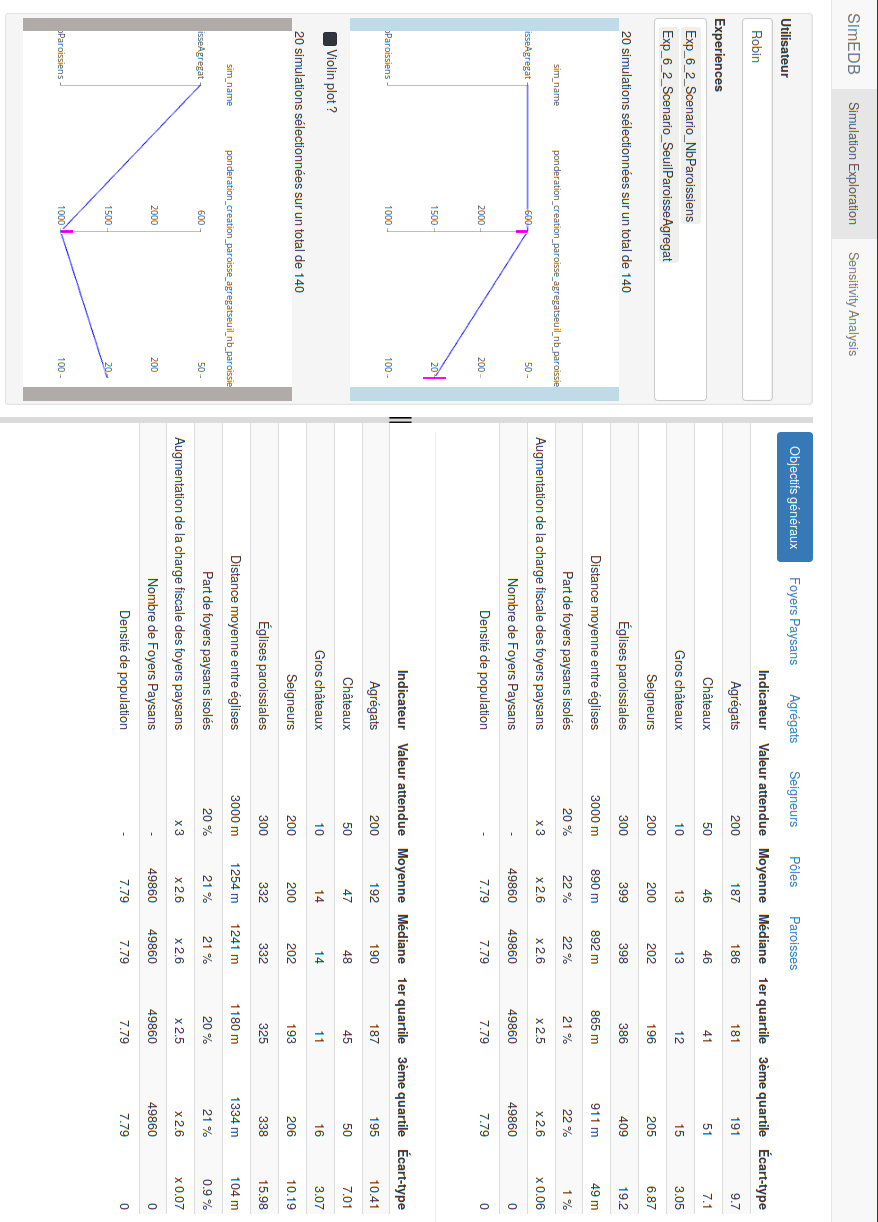
\includegraphics[width=\linewidth]{img/SimEDB_base_rotate.png}
		\caption{SimEDB }
		\label{fig:simedb_villages}
	\end{figure}

	\paragraph*{}
	Nous reviendrons plus précisément et longuement sur la description de SimEDB dans les parties suivantes (\cref{sec:SimEDB}, p. \pageref{sec:SimEDB}), mais après en avoir décrit les étapes de construction et les besoins auxquelles ces évolutions répondaient, il est maintenant nécessaire de revenir sur les données manipulées par cette plate-forme d'exploration.
	Le type, la structure et la masse de ces données (\cref{sec:sorties-simfeodal}) sont en effet indissociables des choix méthodologiques effectués pour SimEDB.
	Il est donc important de présenter les choix et contraintes de ces données avant d'entrer dans une description approfondie de la plate-forme.
